% !Mode:: "TeX:UTF-8"
\chapter{Filters and Optimization Approaches: Part I}
\label{cpt:backend1}
\label{cpt:9}
\begin{mdframed}  
	\textbf{Goal of Study}
	\begin{enumerate}[labelindent=0em,leftmargin=1.5em]
		\item Learn how to formulate the backend problem into a filter or least-square optimization problem.
		\item Learn how to use the sparse structure in the bundle adjustment problem. 
		\item Solve a BA problem with \textit{g2o} and \textit{Ceres}.
	\end{enumerate}
\end{mdframed}

From this lecture, we turn to another important module: backend optimization.
We see that the frontend visual odometry can give a short-term trajectory and map. Still, due to the inevitable accumulation of errors, this map is inaccurate for a long time. Therefore, based on visual odometry, we also hope to construct a larger-scale optimization problem to consider the optimal trajectory and map over a long time. However, considering the balance of accuracy and performance, there are many different approaches in practice.

\newpage
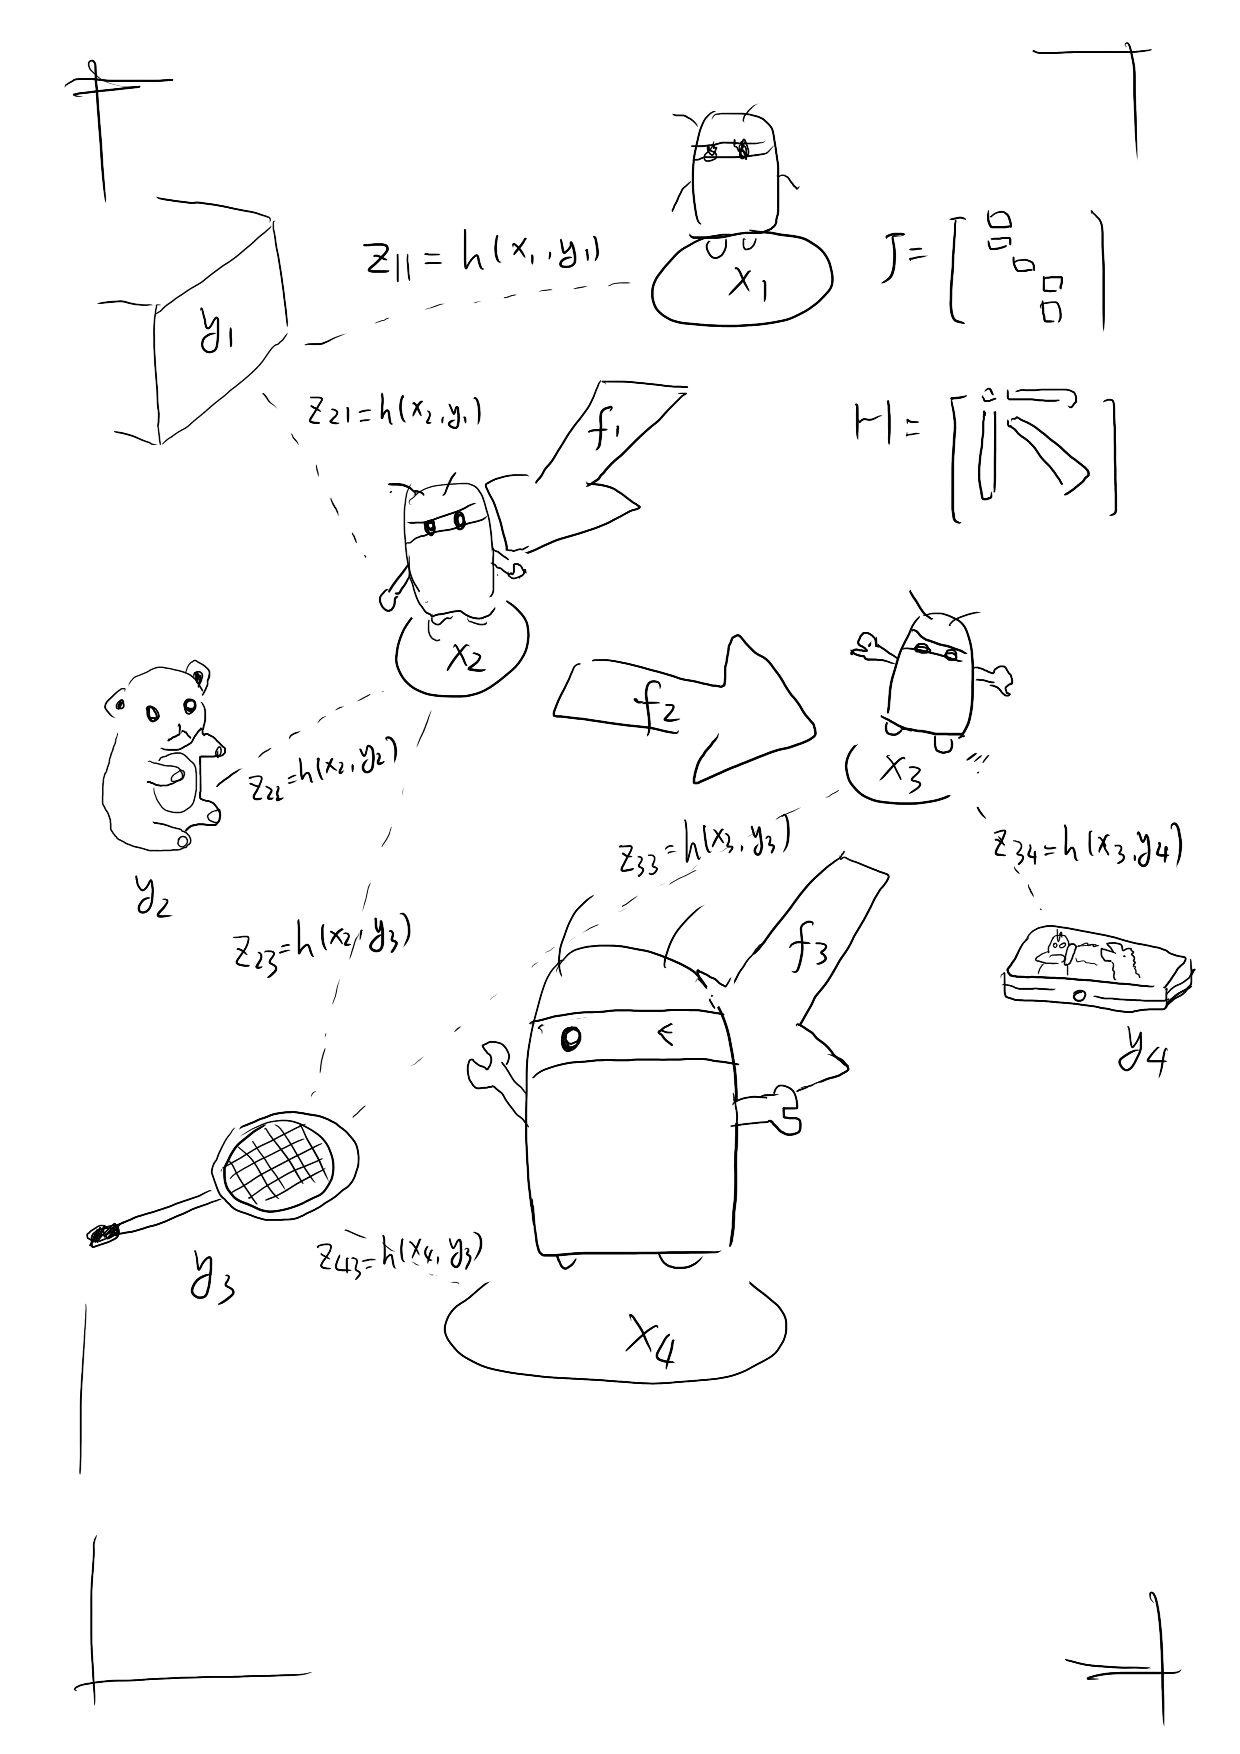
\includepdf{resources/other/ch10.pdf}

\newpage
\section{Introduction}
\subsection{State Estimation from Probabilistic Perspective}
As mentioned in the lecture~\ref{cpt:2}, the visual odometry only has a short memory, but we hope that the system can maintain the entire motion trajectory in an optimal state for a long time. We may use the latest knowledge to update an old state. At that time, it seems that future information tells you, ``where you should be now.'' Therefore, in the backend optimization, we usually consider the problem of state estimation for a longer time (or all-time) and not only use the past information to update our current state but also use future information to update ourselves. Such a method might be called ``batch.'' Otherwise, if the current state is only determined by the past, or even only by the last moment, it might also be called ``incremental.''

We already know that the SLAM process can be described by the motion and observation equations. Suppose in the time from $t=0$ to $t=N$, we have the poses from $\mathbf{x}_0$ to $\mathbf{x}_N$ and observation $\mathbf{y}_1, \cdots, \mathbf{y}_M$. According to the equations in chapter~\ref{cpt:2}, we write them as:
\begin{equation}
	\left\{ \begin{array}{l}
		{\mathbf{x}_k} = f\left( {{\mathbf{x}_{k - 1}},{\mathbf{u}_k}} \right) + \mathbf{w}_k \\
		{\mathbf{z}_{k,j}} = h\left( {{ \mathbf{y}_j},{ \mathbf{x}_k}}  \right)+ \mathbf{v}_{k,j}
	\end{array} \right. \quad k=1, \ldots, N, \  j=1, \ldots, M.
\end{equation}

Note that in the SLAM problem, we have the following characteristics:
\begin{enumerate}
	\item In the observation equation, only when $\mathbf{x}_k$ sees $\mathbf{y}_j$ will we have a real observation equation. In fact, we can usually see only a small part of the landmarks in one location. Moreover, due to a large number of visual SLAM feature points, the number of observation equations in practice will be much larger than that of motion equations.
	\item We may not have a device to measure the motion, so there may not be a motion equation. In this case, there are several ways to deal with it:
	\begin{itemize}
		\item Assume that there is really no motion equation.
		\item Assume that the camera does not move.
		\item Assume that the camera is moving at a constant speed.
	\end{itemize}
	These several methods are all feasible. In the absence of motion equations, the entire optimization problem consists of only observation equations. This is very similar to the SfM (Structure from Motion) problem, which is equivalent to restoring the motion and structure through a set of images. The difference with SfM is that the SLAM images have a chronological order, while SfM allows the use of completely unrelated images.
\end{enumerate} 

We know that every measurement is affected by noise, so the poses $\mathbf{x}$ and landmarks $\mathbf{y}$ here are regarded as \textit{random variables that obey a certain probability distribution} instead of a single number. Therefore, the question becomes: when I have some motion data $\mathbf{u}$ and observation data $\mathbf{z}$, how to determine the state $\mathbf{x}$ and landmarks $\mathbf{y}$'s distribution? Furthermore, if new data is obtained, how to update our estimation? In more common and reasonable cases, we assume that the state quantity and noise terms obey Gaussian distribution-which means that only their mean and covariance matrix need to be stored in the program. The mean can be regarded as an estimate of the state variable's optimal value, and the covariance matrix measures its uncertainty. Then, the question becomes: when there are some motion and observation data, how do we estimate the Gaussian distribution of the states?

We still put ourselves in the role of a robot. When there is only the equation of motion, it is equivalent to walking blindfolded in an unknown place. Although we know how far we have taken each step, we will become more and more uncertain about where we are as time grows. This reflects that when the input data is affected by noise, the error is gradually accumulated, and our estimate of the position variance will become larger and larger. However, when we open our eyes, we will become more confident because we can continuously observe the external scene, making the uncertainty of position estimation smaller. If we use an ellipse to express the covariance matrix intuitively, this process is a bit like walking in a mobile phone map software. Taking \autoref{fig:uncertainty}~ as an example, readers can imagine that when there is no observation data, the circle will become larger and larger with the movement, and if there are correct observations, the circle will shrink to a certain size and keep stable.

\begin{figure}[!ht]
	\centering
	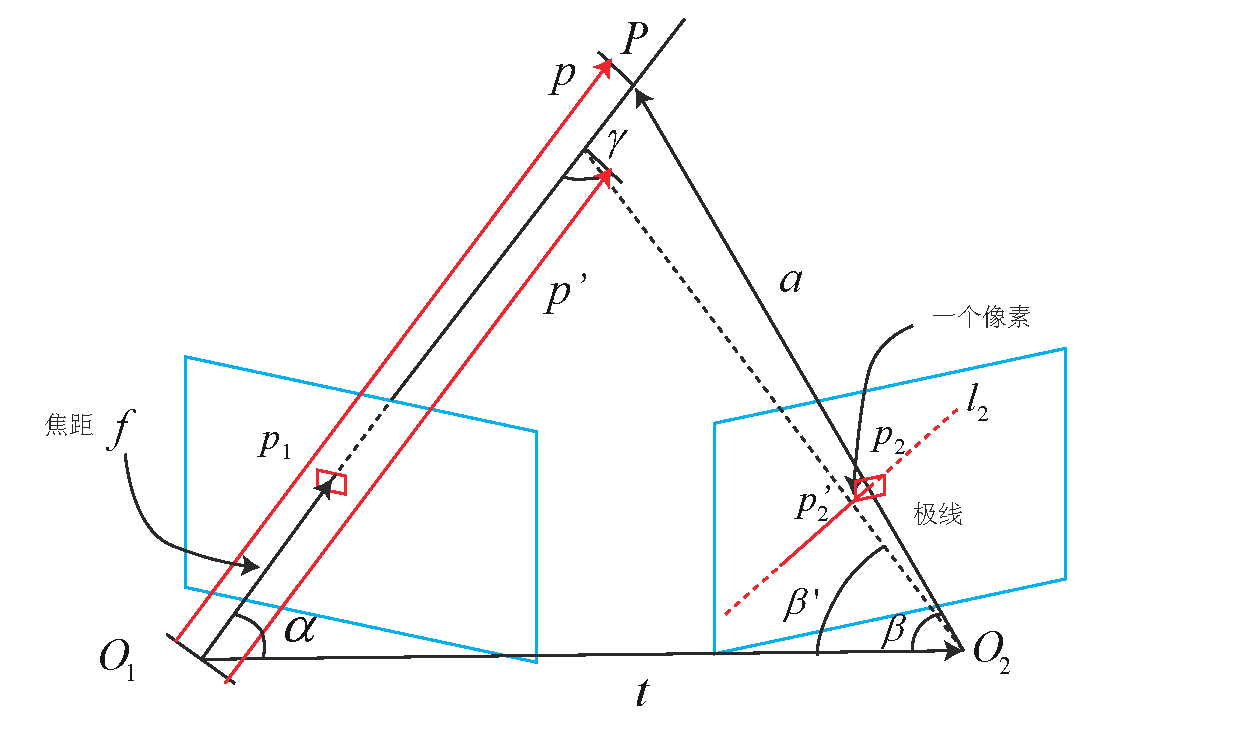
\includegraphics[width=0.66\textwidth]{backend1/uncertainty.pdf}
	\caption{An intuitive description of uncertainty. Left: When there is only the motion equation, the pose at the next moment adds noise to the previous moment, so the uncertainty is getting bigger and bigger. Right: When there are road signs, the uncertainty will be significantly reduced. Please note that this is only an intuitive diagram, not real data.}
	\label{fig:uncertainty}
\end{figure}

The above statements explain the problem of state estimation in a metaphorical form. Below we will look at it in a quantitative way. In lecture~\ref{cpt:6}, we introduced the maximum likelihood estimation where we say that the problem of \textit{batch state estimation} can be transformed into a \textit{maximum likelihood estimation problem} and solved by the \textit{least-square method}. In this section, we will explore how to apply this conclusion to progressive problems and get some classic conclusions. At the same time, we will investigate the special structure of the least-square method in visual SLAM.

First of all, since the poses and landmarks are all optimize variables, we change the notation a bit and let $\mathbf{x}_k$ be all the unknowns at the moment of $k$. It contains the current camera pose and $m$ landmarks. With a little abuse of the notation, we rewrite the equations into:
\begin{equation}
	\mathbf{x}_k  \buildrel \Delta \over =  \{ \mathbf{x}_k, \mathbf{y}_1, \ldots, \mathbf{y}_m \}.
\end{equation}

At the same time, all observations at time $k$ are denoted as $\mathbf{z}_k$. Therefore, we can write the motion and observation equations more concisely. There will be no $\mathbf{y}$ here, but we should remember that the previous $\mathbf{y}$ is already included in the $\mathbf{x}$:
\begin{equation}
	\left\{ \begin{array}{l}
		{\mathbf{x}_k} = f\left( {{\mathbf{x}_{k - 1}},{\mathbf{u}_k}} \right) + \mathbf{w}_k \\
		{\mathbf{z}_{k}} = h\left( \mathbf{x}_k  \right)+ \mathbf{v}_{k}
	\end{array} \right. \quad k=1, \ldots, N .
\end{equation}

Now consider the situation at time $k$. We hope to use the data from $0$ to $k$ to estimate the current state distribution:
\begin{equation}
	P(\mathbf{x}_k | \mathbf{x}_0, \mathbf{u}_{1:k}, \mathbf{z}_{1:k}).
\end{equation}

The subscript $1:k$ represents all the data from time $0$ to time $k$. Please note that $\mathbf{z}_k$ represents all the observation data at time $k$. It may be more than one, but we use a single notation here. At the same time, also note that $\mathbf{x}_k$ is related to the previous states like $\mathbf{x}_{k-1}, \mathbf{x}_{k-2}$, but this formula does not explicitly write them out.

Let's see how to do the state estimation. According to Bayes' rule, swap the positions of $\mathbf{z}_k$ and $\mathbf{x}_k$, we have:
\begin{equation}
	\label{eq:10-5}
	P\left( {{\mathbf{x}_k}|{\mathbf{x}_0},{\mathbf{u}_{1:k}},{\mathbf{z}_{1:k}}} \right) \propto \underbrace{P\left( {{\mathbf{z}_k}|{\mathbf{x}_k}} \right)}_{\text{likelihood}} \underbrace{P\left( {{\mathbf{x}_k}|{\mathbf{x}_0},{\mathbf{u}_{1:k}},{\mathbf{z}_{1:k - 1}}} \right)}_{\text{prior}}.
\end{equation}

You may think this is familiar with what we have discussed in the previous sections. Here the first term is called \textit{likelihood}, and the second term is called \textit{prior}. The observation equation gives the likelihood. For the prior part, we should know that the current state $\mathbf{x}_k$ is estimated based on all past states. Let's first consider the effect of $\mathbf{x}_{k-1}$. It is expanded according to the conditional probability of $\mathbf{x}_{k-1}$ moment:
\begin{equation}
	\label{eq:bayes-estimator}
	\small
	P\left( {{\mathbf{x}_k}|{\mathbf{x}_0},{\mathbf{u}_{1:k}},{\mathbf{z}_{1:k - 1}}} \right) = \int {P\left( {{\mathbf{x}_k}|{\mathbf{x}_{k - 1}},{\mathbf{x}_0},{\mathbf{u}_{1:k}},{\mathbf{z}_{1:k - 1}}} \right)P\left( {{\mathbf{x}_{k - 1}}|{\mathbf{x}_0},{\mathbf{u}_{1:k}},{\mathbf{z}_{1:k - 1}}} \right) \mathrm{d}\mathbf{x}_{k-1} }.
\end{equation}

There are generally some methodology differences for the next steps: (i) We assume the \textit{Markov property}. The simple first-order Markov property assumes that the state at time $k$ is only related to the state at time $k-1$ and is not related to the earlier states. If such an assumption is made, we will get a filter method represented by \textit{Extended Kalman Filter} (EKF). In the filtering method, we estimate from the state at a specific moment and derive it to the next moment. (ii) Another technique is to keep the relationship between the state at $k$ and \textit{all} the previous states (and also, the future states). At this time, we will obtain an optimization framework with \textit{nonlinear optimization} as the main body. The basic knowledge of nonlinear optimization has been introduced in the previous sections. At present, the mainstream of visual SLAM is to use the nonlinear optimization method. However, in order to make this book more comprehensive, let's first introduce the principles of the Kalman filter and EKF.

\subsection{Linear Systems and the Kalman Filter}
Let's look at the filter model first. When the Markov property is assumed, what changes will happen from a mathematical perspective? The current state is only related to the previous moment. The first part on the right side of the formula \eqref{eq:bayes-estimator} can be further simplified as:
\begin{equation}
	P\left( {{\mathbf{x}_k}|{\mathbf{x}_{k - 1}},{\mathbf{x}_0},{\mathbf{u}_{1:k}},{\mathbf{z}_{1:k - 1}}} \right) = P\left( {{\mathbf{x}_k}|{\mathbf{x}_{k - 1}},{\mathbf{u}_k}} \right),
\end{equation}
where we omit the states earlier than $k-1$ since they are not related to the $k$-th state. 

The second part can be simplified as: 
\begin{equation}
	P\left( {{\mathbf{x}_{k - 1}}|{\mathbf{x}_0},{\mathbf{u}_{1:k}},{\mathbf{z}_{1:k - 1}}} \right) = P\left( {{\mathbf{x}_{k - 1}}|{\mathbf{x}_0},{\mathbf{u}_{1:k - 1}},{\mathbf{z}_{1:k - 1}}} \right),
\end{equation}
where we drop the $\mathbf{u}_k$ since it has nothing to do with $\mathbf{x}_{k-1}$. 

It can be seen that this item is actually the state distribution at time $k-1$. Therefore, this series of equations shows that what we are actually doing is ``how to derive the state distribution from time $k-1$ to time $k$''. In other words, we only need to maintain the current state estimation and update it incrementally. Furthermore, if it is assumed that the state quantity obeys a Gaussian distribution, we only need to consider the state variable's mean and covariance. You can imagine that the robot's localization module has been outputting two pieces of information: the estimated pose (mean) and the uncertainty (covariance), which is exactly the common case in many practical localization libraries.

We start from the simplest linear Gaussian system, and finally, we will reach the famous Kalman filter. A linear Gaussian system is such a system where the motion and observation equations are all linear so that we can write them in a matrix form:
\begin{equation}
	\left\{ \begin{array}{l}
		{\mathbf{x}_k} = \mathbf{A}_k {{\mathbf{x}_{k - 1}}+{\mathbf{u}_k}} + \mathbf{w}_k \\
		{\mathbf{z}_{k}} = \mathbf{C}_k  { \mathbf{x}_k} + \mathbf{v}_{k} \end{array} \right. \quad k=1, \ldots, N ,
\end{equation}
and we assume the states and noises are all Gaussian, so that: 
\begin{equation}
	\mathbf{w}_k \sim N(\mathbf{0}, \mathbf{R}). \quad \mathbf{v}_k \sim N( \mathbf{0}, \mathbf{Q}),
\end{equation}
where we omit the subscripts of $\mathbf{R}$ and $\mathbf{Q}$ for brevity. Now, using the Markov property, suppose we know the posterior state estimation at time $k-1$ $\mathbf{\hat{x}}_{k-1} $ and its covariance $\mathbf{\hat{P}}_{k-1}$, now we want to determine the posterior distribution of $\mathbf{x}_k$ based on the input and the observation data at time $k$. In order to distinguish the prior and the posterior variables, we make a difference in the notation: we use the up hat $\mathbf{\hat{x}}_k$ represents the posterior, and use the down hat $\check{\mathbf{x}}_k $ to represent the prior distribution. 

The Kalman filter's first step is to determine the distribution of $\mathbf{x}_k$ through the equation of motion, which is called the prior at time $k$. It is very easy to transform the Gaussians in the linear system: 
\begin{equation}
	P\left( {{\mathbf{x}_k}|{\mathbf{x}_0},{\mathbf{u}_{1:k}},{\mathbf{z}_{1:k - 1}}} \right) = N\left( {\mathbf{A}_k {{\hat{\mathbf{x}}}_{k - 1}} + {\mathbf{u}_k}, \mathbf{A}_k\hat{\mathbf{P}}_{k-1} {\mathbf{A}_k^T} + \mathbf{R}} \right).
\end{equation}

This step is called the \textit{prediction}. Please refer to the appendix~\ref{sec:gauss-example} if you are not familiar with the linear transform here. It shows how to infer the current state distribution based on the noisy input from the previous state. Let's note it as:
\begin{equation}
	\check{\mathbf{x}}_k = {\mathbf{A}_k {{\hat{\mathbf{x}}}_{k - 1}} + {\mathbf{u}_k}}, \quad \check{\mathbf{P}}_k = {\mathbf{A}_k \hat{\mathbf{P}}_{k-1} { \mathbf{A}^T_k} + \mathbf{R}},
\end{equation}
which is very natural. Obviously, the state's uncertainty in this step will become larger because the motion noise is added to our system. On the other hand, from the observation equation, we can calculate what kind of observation data should be generated in a certain state:
\begin{equation}
	P\left( {{\mathbf{z}_k}|{\mathbf{x}_k}} \right) = N\left( {{\mathbf{C}_k}{\mathbf{x}_k},\mathbf{Q}} \right) ,
\end{equation}
which is exactly the likelihood we talked about before. Remember what we want to get is the posterior $P\left( {{\mathbf{x}_k}|{\mathbf{z}_k}} \right) $. In order to do that, we need to calculate the product of the prior and the likelihood according to the Bayesian formula \eqref{eq:10-5}. However, although we know that we will finally get a Gaussian distribution of $\mathbf{x}_k$ in the end, it is a little bit troublesome in the calculation. Let's set the result as $\mathbf{x}_k \sim N(\mathbf{\hat{x}}_k, \mathbf{\hat{P}}_k )$, then:
\begin{equation}
	N(\mathbf{\hat{x}}_k, \mathbf{\hat{P}}_k ) = \eta N\left( {{\mathbf{C}_k}{\mathbf{x}_k},\mathbf{Q}} \right) \cdot N( \mathbf{\check{x}}_k, \mathbf{\check{P}}_k),
\end{equation}
where $\eta$ is a normalization number to make the integral of the distribution equal to one. This is a little tricky method. Please keep in mind that what we really want to know is the relationship between $\hat{\mathbf{x}}_k, \hat{\mathbf{P}}_k$ and $\check{\mathbf{x}}_k, \check{\mathbf{P}}_k$. 

Since we know that both sides of the equation are Gaussian distributions, we only need to compare the exponential part and ignore the factor part in front because they can be merged to $\eta$. The exponential part is very similar to a quadratic form, and let's derive it. First, we expand the exponential part as \footnote{ The the equal sign is not strict here since we can put the variables that are not related to $\mathbf{x}_k$ into $\eta$. }:
\begin{equation}
	\small
	{\left( {{\mathbf{x}_k} - {{\hat{\mathbf{x}}}_k}} \right)^T}\hat{\mathbf{P}}_k^{ - 1}\left( {{\mathbf{x}_k} - {{\hat{\mathbf{x}}}_k}} \right) = {\left( {{\mathbf{z}_k} - {\mathbf{C}_k} {\mathbf{x}_k}} \right)^T}{\mathbf{Q}^{ - 1}}\left( {{\mathbf{z}_k} - {\mathbf{C}_k}{\mathbf{x}_k}} \right) + {\left( {{\mathbf{x}_k} - {{\check{\mathbf{x}}}_k}} \right)^T}\check{\mathbf{P}}_k^{ - 1}\left( {\mathbf{x}_k - {{\check{\mathbf{x}}}_k}} \right).
\end{equation}

In order to compute the $\hat{\mathbf{x}}_k$ with $\mathbf{\hat{P}}_k$ on the left side, we expand the quadratics and compare their first-order and second-order coefficients of $\mathbf{x}_k$. For the second-order coefficients, we have:
\begin{equation}
	\label{eq:kalman-cov}
	\hat{\mathbf{P}}_k^{ - 1} = \mathbf{C}_k^T{\mathbf{Q}^{ - 1}}{\mathbf{C}_k} + \check {\mathbf{P}}_k^{ - 1},
\end{equation}
which gives the relationship of the covariance matrix.

We define an intermediate variable for convenience in the following derivation:
\begin{equation}
	\label{eq:kalman-K}
	\mathbf{K} = \mathbf{\hat{P}}_k \mathbf{C}_k^T \mathbf{Q}^{-1}.
\end{equation}

According to this definition, we multiply $\mathbf{\hat{P}}_k$ on both sides of the equation \eqref{eq:kalman-cov}: 
\begin{equation}
	\mathbf{I} = \mathbf{\hat{P}}_k \mathbf{C}_k^T \mathbf{Q}^{-1} \mathbf{C}_k + \mathbf{\hat{P}}_k \mathbf{\check{P}}_k^{-1} = \mathbf{K} \mathbf{C}_k + \mathbf{\hat{P}}_k \mathbf{\check{P}}_k^{-1}.
\end{equation}

Then we have \footnote{It seems to have a little circular definition here. We define the $\mathbf{K}$ by $\mathbf{\hat{P}}_k$, and then write $\mathbf{\hat{P}}_k$ as the expression of $\mathbf{K}$. However, $\mathbf{K}$ can also be calculated without relying on $\mathbf{\hat{P}}_k$, but this requires the introduction of the Sherman-Morrison-Woodbury identity~\cite{Sherman1950}, see the exercises in this lecture. In practice, we can also simply calculate the $\mathbf{\hat{P}}_k$ first and then use the result to calculate $\mathbf{K}$. }:
\begin{equation}
	\mathbf{\hat{P}}_k = ( \mathbf{I} - \mathbf{K} \mathbf{C}_k ) \mathbf{\check{P}}_k.
\end{equation}

Then we compare the first-order coefficients and get: 
\begin{equation}
	- 2\hat {\mathbf{x}}_k^T \hat{\mathbf{P}}_k^{ - 1}{\mathbf{x}_k} =  - 2\mathbf{z}_k^T {\mathbf{Q}^{ - 1}}{\mathbf{C}_k}{\mathbf{x}_k} - 2\mathbf{\check {x}}_k^T \mathbf{\check {P}}_k^{ - 1}{\mathbf{x}_k}.
\end{equation}

Reorganize it (take the coefficients and transpose them):
\begin{equation}
	\hat { \mathbf{P}}_k^{ - 1}{{\hat{\mathbf{x}}}_k} = \mathbf{C}_k^T {\mathbf{Q}^{ - 1}}{\mathbf{z}_k} + \check{\mathbf{P}}_k^{ - 1}{{\mathbf{\check{x}}}_k}.
\end{equation}

Multiply $\mathbf{\hat{P}}_k$ on both sides and take \eqref{eq:kalman-K} into it:
\begin{align}
	{{\mathbf{\hat {x}}}_k} &= {{\hat {\mathbf{P}}}_k} \mathbf{C}_k^T { \mathbf{Q}^{ - 1}}{\mathbf{z}_k} + {{\mathbf{\hat{ P}}}_k}\check {\mathbf{P}}_k^{ - 1}{{\check {\mathbf{x}}}_k}\\
	&= \mathbf{K} {\mathbf{z}_k} + \left( {\mathbf{I} - \mathbf{K}{\mathbf{C}_k}} \right){{\mathbf{\check {x}}}_k} = {{\check {\mathbf{x}}}_k} + \mathbf{K} \left( {\mathbf{z}_k - {\mathbf{C}_k}{\mathbf{\check{x}}_k}} \right).
\end{align}

So we get the expression of the posterior mean. In summary, the above two steps can be written into two steps:  the ``predict'' and the ``update'':
\begin{mdframed}
	\begin{enumerate}
		\item \textit{Predict}:
		\begin{equation}
			\check{\mathbf{x}}_k = {\mathbf{A}_k {{\hat{\mathbf{x}}}_{k - 1}} + {\mathbf{u}_k}}, \quad \check{\mathbf{P}}_k = {\mathbf{A}_k \hat{\mathbf{P}}_{k-1} { \mathbf{A}^T_k} + \mathbf{R}}.
		\end{equation}
		\item \textit{Update}:
		Calculate $\mathbf{K}$, which is the Kalman gain:
		\begin{equation}
			\label{eq:kalman-K-another}
			\mathbf{K} = {{\check {\mathbf{P}}}_k} \mathbf{C}_k^T {\left( {{\mathbf{C}_k}{{\check {\mathbf{P}}}_k}\mathbf{C}_k^T + {\mathbf{Q}_k}} \right)^{ - 1}},
		\end{equation}
		and the posterior:
		\begin{equation}
			\begin{array}{l}
				\hat {\mathbf{x}}_k = {{\check {\mathbf{x}}}_k} + \mathbf{K} \left( {\mathbf{z}_k - {\mathbf{C}_k}{\mathbf{\check{x}}_k}} \right)\\
				{{\mathbf{\hat {P}}}_k} = \left( {\mathbf{I} - \mathbf{K}{\mathbf{C}_k}} \right) \check{\mathbf{P}}_k.
			\end{array}.
		\end{equation}
	\end{enumerate}
\end{mdframed}

So far, we have derived the classic Kalman filter (to my knowledge, in the simplest way). The Kalman filter has several derivation methods, and we use the form of maximum posterior probability estimation from a probability perspective. We see that in a linear Gaussian system, the Kalman filter constitutes the maximum posterior probability estimate. Moreover, since the Gaussian distribution still obeys the Gaussian distribution after linear transformation, we did not perform any approximation in the whole process. The Kalman filter constitutes the optimal unbiased estimate of the linear system. If readers are interested in other derivation methods, please refer to the state estimation books like~\cite{Barfoot2016}.

\subsection{Nonlinear systems and the EKF}
After introducing the Kalman filter, we must clarify one point: the motion equation and observation equation in SLAM are usually nonlinear functions, especially the camera model in visual SLAM, which requires the camera projection model and the pose represented by $\mathrm{SE}(3)$.  A Gaussian distribution, after a nonlinear transformation, is often no longer Gaussian. Therefore, in a nonlinear system, we must take a certain approximation to transform the non-Gaussian distributions into Gaussians. 

If we hope to extend the Kalman filter results to a nonlinear system, we will get an Extended Kalman Filter (EKF). The usual approach is to consider the first-order Taylor expansion of the motion equation and the observation equation near a certain point (working point), and only retain the first-order term, that is, the linear part, and then derive it according to the linear system. 

Let's do the derivation just like for the Kalman filter. Let the mean and covariance matrix at time $k-1$ be $\mathbf{\hat{x}}_{k-1},\mathbf{\hat{P}}_{k-1}$. At the moment $k$, we put the motion equation and the observation equation at $\mathbf{\hat{x}}_{k-1},\mathbf{\hat{P}}_{k-1}$, and do the \textit{linearization} (equivalent to first-order Taylor expansion):
\begin{equation}
	{\mathbf{x}_k} \approx f\left( {{{\mathbf{\hat x}}_{k - 1}},{\mathbf{u}_k}} \right) + {\left. {\frac{{\partial f}}{{\partial {\mathbf{x}_{k - 1}}}}} \right|_{{{\mathbf{\hat x}}_{k - 1}}}}\left( {{\mathbf{x}_{k - 1}} - {{\mathbf{\hat x}}_{k - 1}}} \right) + {\mathbf{w}_k}.
\end{equation}

Note the partial derivative here as:
\begin{equation}
	\mathbf{F} = \left. {\frac{{\partial f}}{{\partial {\mathbf{x}_{k - 1}}}}} \right|_{{{\mathbf{\hat x}}_{k - 1}}}.
\end{equation}

Similar for the observation model:
\begin{equation}
	{\mathbf{z}_k} \approx h\left( {{{\mathbf{\check x}}_k}} \right) + {\left. {\frac{{\partial h}}{{\partial {\mathbf{x}_k}}}} \right|_{{{\mathbf{\check x}}_k}}}\left( {\mathbf{x}_k - {{\mathbf{\check x}}_k}} \right) + {\mathbf{n}_k}.
\end{equation}

And note the partial derivative as:
\begin{equation}
	\mathbf{H} = \left. {\frac{{\partial h}}{{\partial {\mathbf{x}_k}}}} \right|_{{{\mathbf{\check x}}_k}}.
\end{equation}

Then the \textit{prediction} part becomes:
\begin{equation}
	P\left( {{\mathbf{x}_k}|{\mathbf{x}_0},{\mathbf{u}_{1:k}},{\mathbf{z}_{0:k - 1}}} \right)
	= N(f\left( {{{\mathbf{\hat x}}_{k - 1}},{\mathbf{u}_k}} \right), \mathbf{F}\mathbf{\hat{P}}_{k-1} \mathbf{F}^T + \mathbf{R}_k),
\end{equation}
which is almost same as the Kalman filter. We note the prior mean and covariance as:
\begin{equation}
	\mathbf{\check {x}}_k = f\left( {{{\mathbf{\hat x}}_{k - 1}},{\mathbf{u}_k}} \right), \quad \mathbf{\check{P}}_k = \mathbf{F}\mathbf{\hat{P}}_{k-1} \mathbf{F}^T + \mathbf{R}_k.
\end{equation}

Then, for the observation part, we have: 
\begin{equation}
	P\left( {{\mathbf{z}_k}|{\mathbf{x}_k}} \right) = N( h\left( {{{\mathbf{\check x}}_k}} \right) + \mathbf{H} \left( {\mathbf{x}_k - {{\mathbf{\check x}}_k}} \right), \mathbf{Q}_k ).
\end{equation}

Finally, according to the Bayesian formula, the posterior probability form of $\mathbf{x}_k$ can be derived. We omit the intermediate derivation process and only give the results. Readers can imitate the Kalman filter to derive the EKF prediction and update equations. In short, we will first define a \textit{Kalman gain} $\mathbf{K}_k$:

\begin{equation}
	\mathbf{K}_k = {\mathbf{\check{P}}_{k}}{\mathbf{H}^T}{\left( {\mathbf{H}{\mathbf{\check P}_k}{\mathbf{H}^T} + {\mathbf{Q}_k}} \right)^{ - 1}}.
\end{equation}

The posterior can be written out based on the $\mathbf{K}$: 
\begin{equation}
	{{\mathbf{\hat x}}_k} = {{\mathbf{\check x}}_k} + {\mathbf{K}_k}\left( {{\mathbf{z}_k} - h\left( {{\mathbf{\check x}_k}} \right)} \right),{\mathbf{\hat P}_k} = \left( {\mathbf{I} - {\mathbf{K}_k}{\mathbf{H}}} \right) \mathbf{\check{P}}_k.
\end{equation}

The EKF shows the change of the state variable distribution after linearization. In the linear system and Gaussian noise case, the Kalman filter gives an unbiased optimal estimate. In nonlinear systems like SLAM, it gives the maximum a posteriori estimate (MAP) under a single linearization step. 

\subsection{Discussion about KF and EKF}
EKF is known for its simple form and wide application. It may seem to be a bit complicated at first glance, but you find it is really very easy to implement (less than 20 lines in Python or MATLAB).  When we want to estimate a certain amount of uncertainty within a certain period of time, the first thing we think of is the EKF. In the early SLAM researches, EKF occupied a dominant position for a long time. Researchers implemented a lot of various filters in SLAM, such as IF (information filter) {\cite{Sujan2005} }, IKF {\cite{Janabi-Sharifi2010}} (Iterated KF), UKF {\cite{Li2010}} (Unscented KF) and particle filter~\cite{Sim2007, Lee2011, Gil2010a}, SWF (Sliding Window \mbox{Filter) {\cite{Sibley2010}}}, etc. {\cite{Chen2012}} \footnote{The principle of particle filter is quite different from Kalman filter. }, or use divide and conquer to improve the efficiency of EKF {\cite{Paz2008, Grasa2011}}. To this day, although we realize that nonlinear optimization has obvious advantages over filters, EKF is still an effective way when the computing resources are limited, or the state dimension is relatively small.

So, is EKF enough for modern SLAM systems? Why are we using optimization approaches rather than the filters? The issues come from two aspects: the theoretical and practical. 


\begin{enumerate}
	\item 
	First of all, the filter method always assumes a certain extent Markov property: the $k$-th state is only related to $k-1$ (or finite moments before). It is not related to the state and observations before $k-1$. This is like considering only the relationship between two adjacent frames in visual odometry. If the current frame is indeed related to data long ago (for example, the robot returns to the origin after a long time), the filter method will be difficult to process in such cases.
	
	The optimization methods tend to use longer or all historical data. It not limited feature points and trajectories at adjacent moments but also considers the long ago states, which is called the Full-SLAM. In this sense, nonlinear optimization methods use more information and, of course, require more calculations.
	
	\item 
	Compared with the optimization method introduced in Lecture 6, the EKF filter is only linearized \textit{once} at $\mathbf{\hat{x}}_{k-1}$. Then we calculated the posterior directly based on the linearization result at this time. This is equivalent to saying that we believe that the linear approximation is still valid at the posterior point. In fact, when we are far away from the operating point, the first-order Taylor expansion may not be able to approximate the entire function, which depends on the nonlinearity of the motion model and the observation model. If they have a strong nonlinearity, then the linear approximation is only valid in a small range, and we cannot consider that the linear approximation can still be used at a long distance. This is known as the \textit{nonlinear error} of EKF and is also a major problem.
	
	In the optimization problem, although we also make the first-order (fastest descent) or second-order (Gauss-Newton method or Levenberg-Marquardt method) approximation, after each iteration, we will re-do the Taylor expansion for the new estimated point, instead of only doing it once on a fixed point like EKF. This makes the optimization method applicable to a wider range, which can also be effective when the state changes greatly. So, in general, you can roughly think that \textit{EKF is just one iteration of optimization}\footnote{Technically, it is better than one iteration because the linearization of the update step is based on prediction. If the motion and observation model is linearized simultaneously at the time of prediction, it is the same as an iteration in the optimization. }.
	
	\item 
	From the point of view of implementation, EKF needs to store the state variable's mean and variance in the memory and update them iteratively. If the landmarks are also put into the states, where the number of landmarks is significantly larger than that of the poses in visual SLAM, this storage amount is considerable, and it grows squarely with the state amount (because the covariance matrix is also stored). Therefore, it is generally believed that EKF SLAM is not suitable for large-scale scenarios.
	
	\item 
	Finally, filter methods such as EKF have no outlier detection mechanism, which causes the system to diverge when there are outliers. Outliers are very common in visual SLAM: regardless of feature matching or optical flow method, it is easy to track or match to the wrong point. Lack of an outlier detection mechanism will make the system very unstable in practice.
\end{enumerate}

Due to these obvious shortcomings of EKF, we usually think that with the same amount of calculation, nonlinear optimization can achieve better results than the filters in terms of accuracy and robustness  {\cite{Strasdat2012}}. Let's discuss the backend based on nonlinear optimization in the following sections. We will mainly introduce the graph optimization and demonstrate the backend optimization with \textit{g2o} and \textit{Ceres}.

\section{Bundle Adjustment and Graph Optimization}
If you have been working on visual 3D reconstruction, you should be familiar with this concept. The so-called Bundle Adjustment refers to optimizing both camera parameters (intrinsic and extrinsic) and 3D landmarks with images. Consider the bundles of light rays emitted from 3D points. They are projected into the image planes of several cameras and then detected as feature points. The purpose of optimization can be explained as to \textit{adjust} the camera poses and the 3D points, to ensure the projected 2D features (bundles) match the detected results {\cite{Triggs2000}}.

We have briefly introduced the principles of BA in lectures~\ref{cpt:5} and~\ref{cpt:7}. This section aims to introduce the characteristics of its corresponding graph model structure and then introduce some general quick solutions.

\subsection{The Projection Model and Cost Function}
First, let's review the entire projection process. Starting from a point $\mathbf{p}$ in the world coordinate system, taking into account the internal and external parameters and distortion of the camera, and finally projecting into pixel coordinates, we get the following steps.

\begin{enumerate}
	\item First, transform the world coordinates into the camera frame using extrinsics $(\mathbf{R}, \mathbf{t})$:
	\begin{equation}
		\mathbf{P}' = \mathbf{R} \mathbf{p} + \mathbf{t} = [X', Y', Z']^T.
	\end{equation}
	\item Then, project $\mathbf{P}'$ into the normalized plane and get the normalized coordinates: 
	\begin{equation}
		\mathbf{P}_c = [u_c, v_c, 1]^T = [X'/Z', Y'/Z', 1]^T.
	\end{equation}
	\item Apply the distortion model. We only consider the radical distortion here: 
	\begin{equation}
		\left\{
		\begin{array}{l}
			u_c' = {u_c}\left( {1 + {k_1}r_c^2 + {k_2}r_c^4} \right)\\
			v_c' = {v_c}\left( {1 + {k_1}r_c^2 + {k_2}r_c^4} \right)
		\end{array}
		\right. .
	\end{equation}
	\item And compute the pixel coordinates using intrinsics:
	\begin{equation}
		\left\{ \begin{array}{l}
			{u_s} = {f_x}u_c' + {c_x}\\
			{v_s} = {f_y}v_c' + {c_y} 
		\end{array} \right. .
	\end{equation}
\end{enumerate}

This series of calculation procedures seems a bit long for beginners. We use the process \autoref{fig:calculationflow}~ to visualize the entire process to help readers understand. Readers should be able to understand that this process is exactly the \textit{observation equation} mentioned earlier, and we note it as:
\begin{equation}
	\mathbf{z} = h(\mathbf{x}, \mathbf{y}).
\end{equation}

\begin{figure}[!htp]
	\centering
	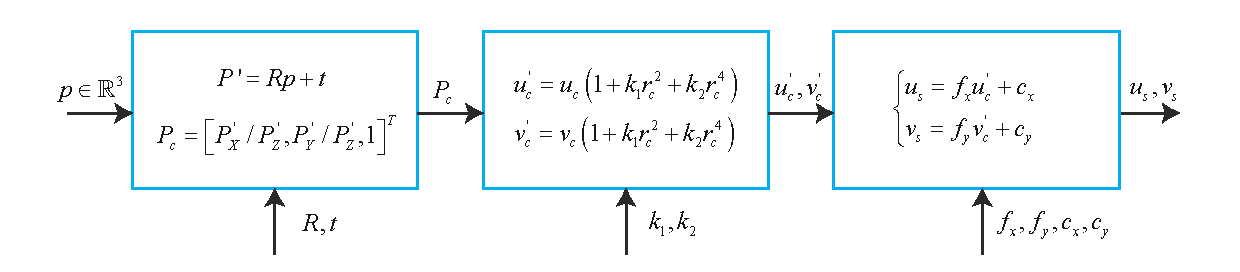
\includegraphics[width=1.0\textwidth]{backend1/calculationflow}
	\caption{Schematic diagram of the calculation process. The $\mathbf{p}$ on the left is the 3D point in the world frame, and the $u_s, v_s$ on the right are the final pixel coordinates of the point on the image plane. $r_c^2=u_c^2 + v_c^2$ in the intermediate distortion model.}
	\label{fig:calculationflow}
\end{figure}


Now, we give its detailed parameterization process. Specifically, the $\mathbf{x}$ here refers to the pose of the camera. We may write it as $\mathbf{R}, \mathbf{t}$, or $\mathbf{T }$ in the corresponding Lie group, or the  Lie algebra $\mathbf{\xi}$. The landmark $\mathbf{y}$ is the three-dimensional point $\mathbf{p}$ here, and the observation data is the pixel coordinate $\mathbf{z} \buildrel \Delta \over = [u_s, v_s]^T $. Consider from the perspective of least-squares, and we can write out the error of this observation:
\begin{equation}
	\mathbf{e} = \mathbf{z} - h(\mathbf{T}, \mathbf{p}).
\end{equation}

Then, let's consider the observations at other moments by adding a subscript to the error. Suppose $\mathbf{z}_{ij}$ is the data generated by observing landmark $\mathbf{p}_j$ at the pose $\mathbf{T}_i$, then the overall \textit{cost function} is:
\begin{equation}
	\label{eq:BAcostfunction}
	\frac{1}{2}\sum_{i=1}^m \sum_{j=1}^n \| \mathbf{e}_{ij} \|^2 = \frac{1}{2}\sum_{i=1}^m\sum_{j=1}^n \|
	\mathbf{{z}}_{ij} - h(\mathbf{T}_{i},\mathbf{p}_j) \|^2 .
\end{equation}


Solving this least-squares is equivalent to adjusting the pose and road signs at the same time, which is the so-called BA. Next, we will gradually discuss the solution of the model based on the objective function and the nonlinear optimization content introduced in the lecture~\ref{cpt:6}.

\subsection{Solving Bundle Adjustment}
Looking into the observation model $h(\mathbf{T}, \mathbf{p})$ in the previous section, it is easy to tell that the function is not a linear function. So we hope to use some nonlinear optimization methods introduced in section~\ref{sec:6.2} to optimize it. According to the principle of nonlinear optimization, we should start from a certain initial value and continuously look for the descending direction $\Delta \mathbf{x}$ to find the optimal solution of the objective function, that is, continuously solve the incremental equation \eqref{eq:minimize-deltax} for the increment $\Delta \mathbf{x}$. Although a single error term is only for one pose and one landmark, the overall BA is about optimizing all variables together:
\begin{equation}
	\mathbf{x} = [ \mathbf{T}_1, \ldots, \mathbf{T}_m, \mathbf{p}_1, \ldots, \mathbf{p}_n ]^T.
\end{equation}

Correspondingly, the $\Delta \mathbf{x}$ in the increment equation is the increment of the overall variable. In this sense, when we give an increment to the optimization variable, the objective function becomes
\begin{equation}
	\label{eq:tangentbundleindetail}
	\frac{1}{2}\left\Vert f(\mathbf{x} + \Delta \mathbf{x}) \right\Vert ^2 \approx \frac{1}{2}\sum_{i=1}^{m}\sum_{j=1}^n \left\Vert \mathbf{e}_{ij} + \mathbf{F}_{ij} \Delta \mathbf{\xi}_{i} + \mathbf{E}_{ij} \Delta \mathbf{p}_j \right\Vert^2,
\end{equation}
where $\mathbf{F}_{ij}$ is the partial derivative of the entire cost function to the $i$-th pose, and $\mathbf{E}_{ij}$ is the partial derivative of the function to the $j$-th landmark. We have introduced their specific forms in the ~\ref{sec:BA-vo1}~ section, so we will not expand the derivation here. Now, put the camera pose variables together:
\begin{equation}
	\mathbf{x}_c=[ \mathbf{\xi}_1, \mathbf{\xi}_2, \ldots, \mathbf{\xi}_m ]^T \in \mathbb{R}^{6m},
\end{equation}
and also the landmarks together: 
\begin{equation}
	\mathbf{x}_p=[ \mathbf{p}_1, \mathbf{p}_2, \ldots , \mathbf{p}_n ]^T\in \mathbb{R}^{3n},
\end{equation}
then the equation \eqref{eq:tangentbundleindetail} can be simplified as: 
\begin{equation}
	\label{eq:BAleastsquare}
	\frac{1}{2}
	\left\Vert 
	f(\mathbf{x}+ \Delta \mathbf{x} )
	\right\Vert ^2 = 
	\frac{1}{2} 
	\left\Vert 
	\mathbf{e} + \mathbf{F}\Delta \mathbf{x}_c + \mathbf{E} \Delta \mathbf{x}_p 
	\right \Vert ^2 .
\end{equation}

It should be noted that this formula has changed from a sum of many small quadratic terms to a more overall form (sometimes mentioned as the ``lifted form''). The Jacobian matrix $\mathbf{E}$ and $\mathbf{F}$ in this equation are the derivative of the overall objective function to the overall variable. It will be a large matrix that are patched by many small blocks like $\mathbf{F}_{ij}$ and $\mathbf{E}_{ij}$ from individual error terms. Then, whether we use the Gauss Newton method or the Levenberg-Marquardt method, we will finally face the incremental linear equation:
\begin{equation}
	\mathbf{H} \Delta \mathbf{x} = \mathbf{g}.
\end{equation}

According to the knowledge of~\ref{cpt:6}, we know that the main difference between the Gauss Newton method and the Levenberg-Marquardt method is that the $\mathbf{H}$ here is taken from $\mathbf{J }^T\mathbf{J}$ or $\mathbf{J}^T\mathbf{J}+ \lambda \mathbf{I}$. Since we have categorized the variables into poses and landmarks, the Jacobian matrix can be divided into two parts:
\begin{equation}
	\mathbf{J}=[\mathbf{F} \ \mathbf{E}].
\end{equation}

So the Hessian matrix will be (take Gauss-Newton as an example): 
\begin{equation}\label{eq:HessianMatrix}
	\mathbf{H} = \mathbf{J}^T\mathbf{J} =
	\begin{bmatrix}
		\mathbf{F}^T\mathbf{F}   &   \mathbf{F}^T\mathbf{E}   \\ 
		\mathbf{E}^T\mathbf{F}   &   \mathbf{E}^T\mathbf{E}
	\end{bmatrix} .
\end{equation}

Of course, in the Levenberg-Marquardt method we also need to calculate this matrix. It is not difficult to find that the dimension of this linear equation will be very large because all optimization variables are considered, including all camera poses and landmarks. Especially in visual SLAM, a single image will contain hundreds of feature points, which greatly increases the dimension of this linear equation. If we directly invert $\mathbf{H}$ to solve the incremental equation, such a matrix inversion is an operation ~\cite{Sueli2003} with $O(n^3)$ complexity, which is very expensive in computation. Fortunately, the $\mathbf{H}$ matrix here has a certain special structure. Using this special structure, we can speed up the solution process.

\subsection{Sparsity}
An important development of visual SLAM in the 21st century is to recognize the sparse structure of the matrix $\mathbf{H}$, and find that this structure can be naturally and explicitly represent by a graph  {\cite{Kummerle2011, Polok2013}}. This section will discuss the matrix sparse structure in detail.

The sparsity of the $\mathbf{H}$ matrix is caused by the Jacobian matrix $\mathbf{J}(\mathbf{x})$. Consider one of the error terms $\mathbf{e}_{ij}$. Note that this error term only describes the residual about $\mathbf{p}_j$ in $\mathbf{T}_i$, and only involves the $i$-th camera pose and the $j$-th landmark. The derivatives of the remaining variables are all 0. Therefore, the Jacobian matrix corresponding to the error term has the following form:
\begin{equation}
	\mathbf{J}_{ij}(\mathbf{x}) = \left(
	\mathbf{0}_{2 \times 6},...
	\mathbf{0}_{2 \times 6},
	\frac{\partial \mathbf{e}_{ij}}{\partial \mathbf{T}_i},
	\mathbf{0}_{2 \times 6},...
	\mathbf{0}_{2 \times 3},...
	\mathbf{0}_{2 \times 3},
	\frac{\partial \mathbf{e}_{ij}}{ \partial \mathbf{p}_j},
	\mathbf{0}_{2 \times 3},...
	\mathbf{0}_{2 \times 3} 
	\right) ,
\end{equation}
where $\mathbf{0}_{2 \times 6}$ represents the $\mathbf{0}$ matrix with dimension $2 \times 6$, and the same for $\mathbf{0}_{2 \times 3}$. The partial derivative of the error term to the camera pose ${\partial \mathbf{e}_{ij}}/{\partial \mathbf{\xi}_i}$ has a dimension of $2 \times 6$, and the partial derivative of the landmark ${\partial \mathbf{e}_{ij}}/{\partial \mathbf{p}_j}$ dimension is $2 \times 3$. The Jacobian matrix of this error term is zero except for the two non-zero blocks. This reflects the fact that the error term has nothing to do with other landmarks and poses except $\mathbf{T}_i$ and $\mathbf{p}_j$. From the perspective of graph optimization, this observation edge is only related to two vertices. So, how does it affect the incremental equation? Why does the $\mathbf{H}$ matrix have sparsity?

\begin{figure}[!htp]
	\centering
	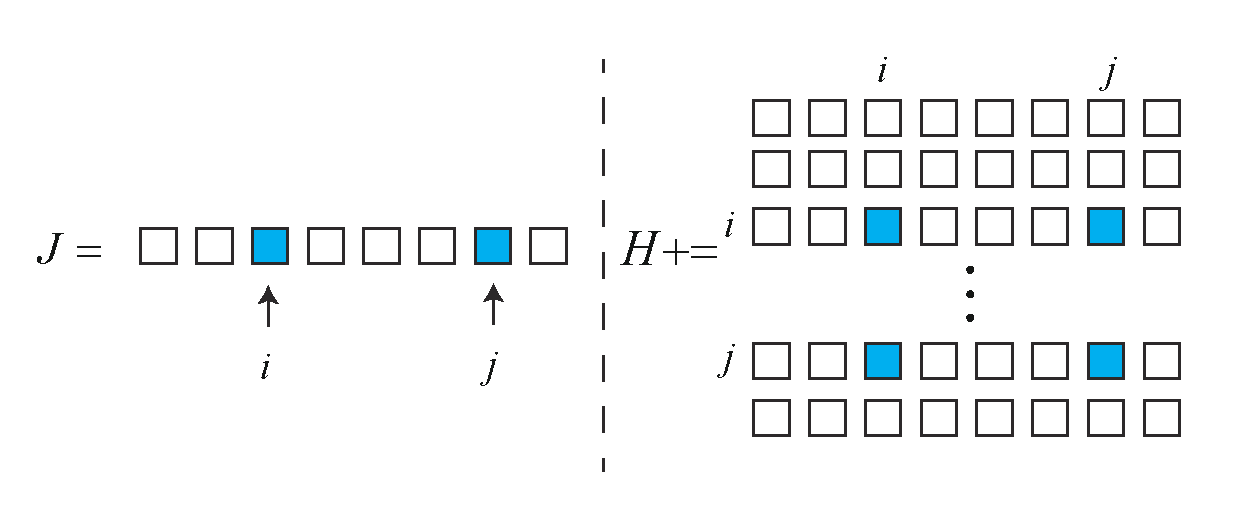
\includegraphics[width=1.0\textwidth]{backend1/sparse.pdf}
	\caption{When an error term has sparsity in its Jacobian $\mathbf{J}$, it will also contribute to the sparsity of the Hessian $\mathbf{H}$.}
	\label{fig:sparse}
\end{figure}

Let's look and the example of ~\autoref{fig:sparse}. Since $\mathbf{J}_{ij}$ only has non-zero blocks in column $i, j$, it will add four non-zero blocks into the overall Hessian matrix $\mathbf{H}$. The non-zero blocks are at $(i,i), (i,j), (j,i), (j,j)$: 
\begin{equation}
	\mathbf{H} = \sum_{i,j} \mathbf{J}_{ij}^T \mathbf{J}_{ij},
\end{equation}

Now let's divide $\mathbf{H}$ into blocks: 
\begin{equation}
	\label{eq:H-blocks}
	\mathbf{H} = \left[ {\begin{array}{*{20}{c}}
			{{\mathbf{H}_{11}}}&{{\mathbf{H}_{12}}}\\
			{{\mathbf{H}_{21}}}&{{\mathbf{H}_{22}}}
	\end{array}} \right] .
\end{equation}
where $\mathbf{H}_{11}$ is only related to camera poses and $\mathbf{H}_{22}$ only to landmarks. When we iterate over the $i,j$ index, please note that the following properties are always hold:
\begin{enumerate}
	\item No matter how $i,j$ changes, $\mathbf{H}_{11}$ is always a block-diagonal matrix, with only non-zero blocks at $\mathbf{H}_{i,i}$.
	\item Save for $\mathbf{H}_{22}$ since we only have non-zero blocks in $\mathbf{H}_{j,j}$. 
	\item  For $\mathbf{H}_{12}$ and $\mathbf{H}_{21}$, they may be sparse or dense, depending on the specific observation data.
\end{enumerate}
This shows the sparse structure of $\mathbf{H}$. We will take advantage tof the sparsity in following section to solve the incremental equations. 

\subsection{Minimal Example of BA}
Let us give an example to illustrate the situation intuitively. Suppose there are two camera poses ($C_1, C_2$) and six landmarks ($P_1, P_2, P_3, P_4, P_5, P_6$) in the scene. The variables corresponding to these cameras and point clouds are $\mathbf{T}_i, i = 1,2$ and $\mathbf{p}_j, j = 1,\cdots, 6$. The camera $C_1$ observes the landmarks $P_1, P_2, P_3, P_4$, and the camera $C_2$ observes $P_3, P_4, P_5, P_6$. We draw this process as a schematic \autoref{fig:simplegraph}~. Cameras and landmarks are represented by circular nodes. If the $i$-th camera can observe the $j$-th point, we will connect an edge at their corresponding node.

\begin{figure}[!htp]
	\centering
	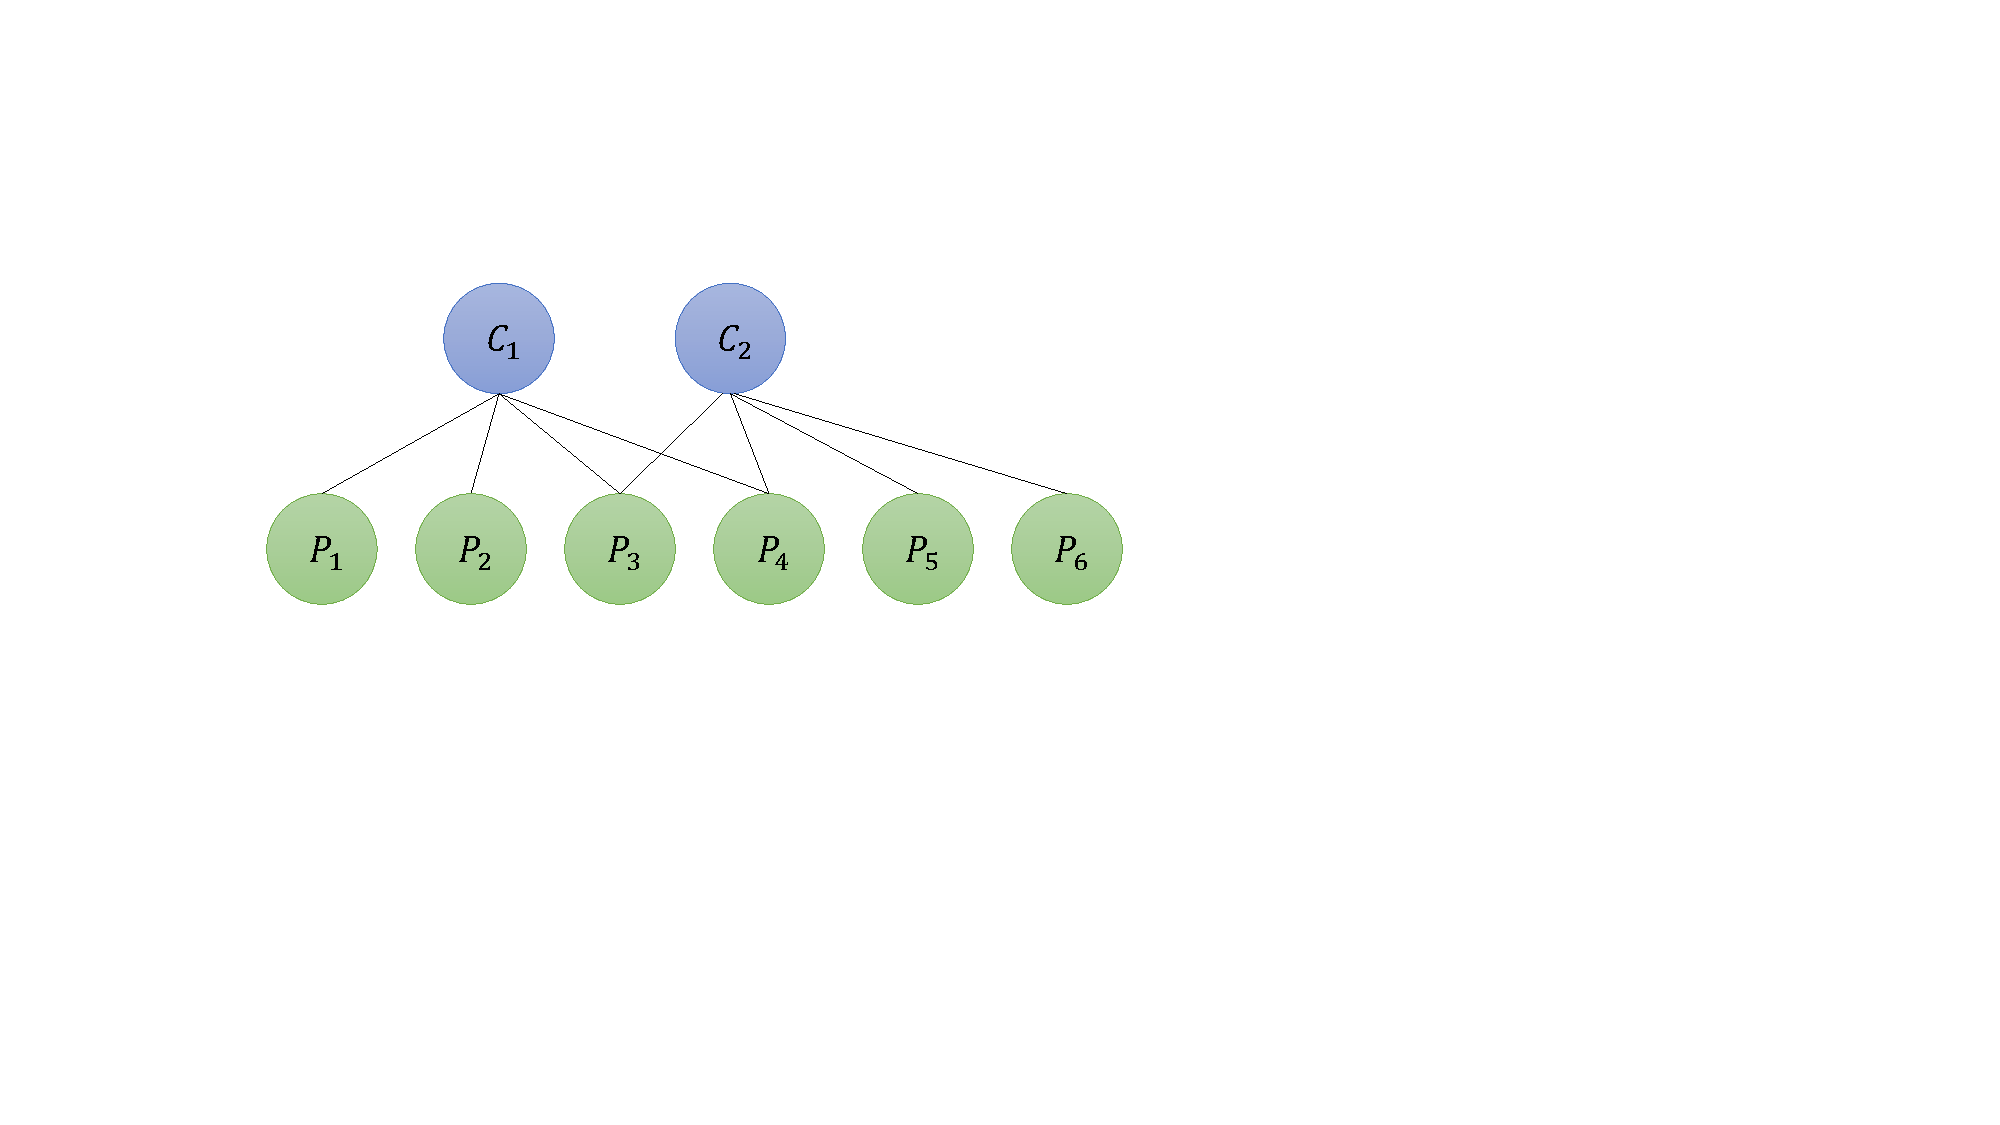
\includegraphics[width=0.8\textwidth]{backend1/simplegraph.pdf}
	\caption{A minimal example of bundle adjustment. }
	\label{fig:simplegraph}
\end{figure}

We can easily write out the overall cost function as: 
\begin{equation}
	\frac{1}{2}\left( \left\Vert \mathbf{e}_{11} \right\Vert^2 + 
	\left\Vert \mathbf{e}_{12} \right\Vert^2 + 
	\left\Vert \mathbf{e}_{13} \right\Vert^2 + 
	\left\Vert \mathbf{e}_{14} \right\Vert^2 + 
	\left\Vert \mathbf{e}_{23} \right\Vert^2 + 
	\left\Vert \mathbf{e}_{24} \right\Vert^2 + 
	\left\Vert \mathbf{e}_{25} \right\Vert^2 + 
	\left\Vert \mathbf{e}_{26} \right\Vert^2 
	\right).
\end{equation}

Here, the $\mathbf{e}_{ij}$ follows the previous definition of \eqref{eq:BAcostfunction}. Take $\mathbf{e}_{11}$ as an example. It describes observation of $P_1$ in $C_1$, which has nothing to do with other camera poses and landmarks. Let $\mathbf{J}_{11}$ be the Jacobian matrix corresponding to $\mathbf{e}_{11}$, and it is not difficult to see that the partial derivatives of $\mathbf{\xi}_2$ and landmarks $\mathbf{p}_2, \cdots, \mathbf{p}_6$ are all zero. We rearrange the variables in the order of $\mathbf{x} = \left( \mathbf{\xi}_1, \mathbf{\xi}_2, \mathbf{p}_1, \cdots, \mathbf{p}_2 \right)^T$,  then we have: 
\begin{equation}
	\mathbf{J}_{11} = \frac{\partial \mathbf{e}_{11}}{\partial \mathbf{x}}
	= \left(
	\frac{\partial \mathbf{e}_{11}}{\partial \mathbf{\xi}_1},
	\mathbf{0}_{2\times 6},
	\frac{\partial \mathbf{e}_{11}}{\partial \mathbf{p}_1},
	\mathbf{0}_{2\times 3},
	\mathbf{0}_{2\times 3},
	\mathbf{0}_{2\times 3},
	\mathbf{0}_{2\times 3},
	\mathbf{0}_{2\times 3}
	\right).
\end{equation}

In order to show the sparsity, we use a colored square to indicate that the matrix has a non-zero value in the square, and the remaining areas without color indicate that the matrix has a value of 0 at that place. Then the above $\mathbf{J}_{11}$ can be expressed as the pattern shown in \autoref{fig:jaobianrow}~. Similarly, other Jacobian matrices will have similar sparse patterns.

\begin{figure}[!t]
	\centering
	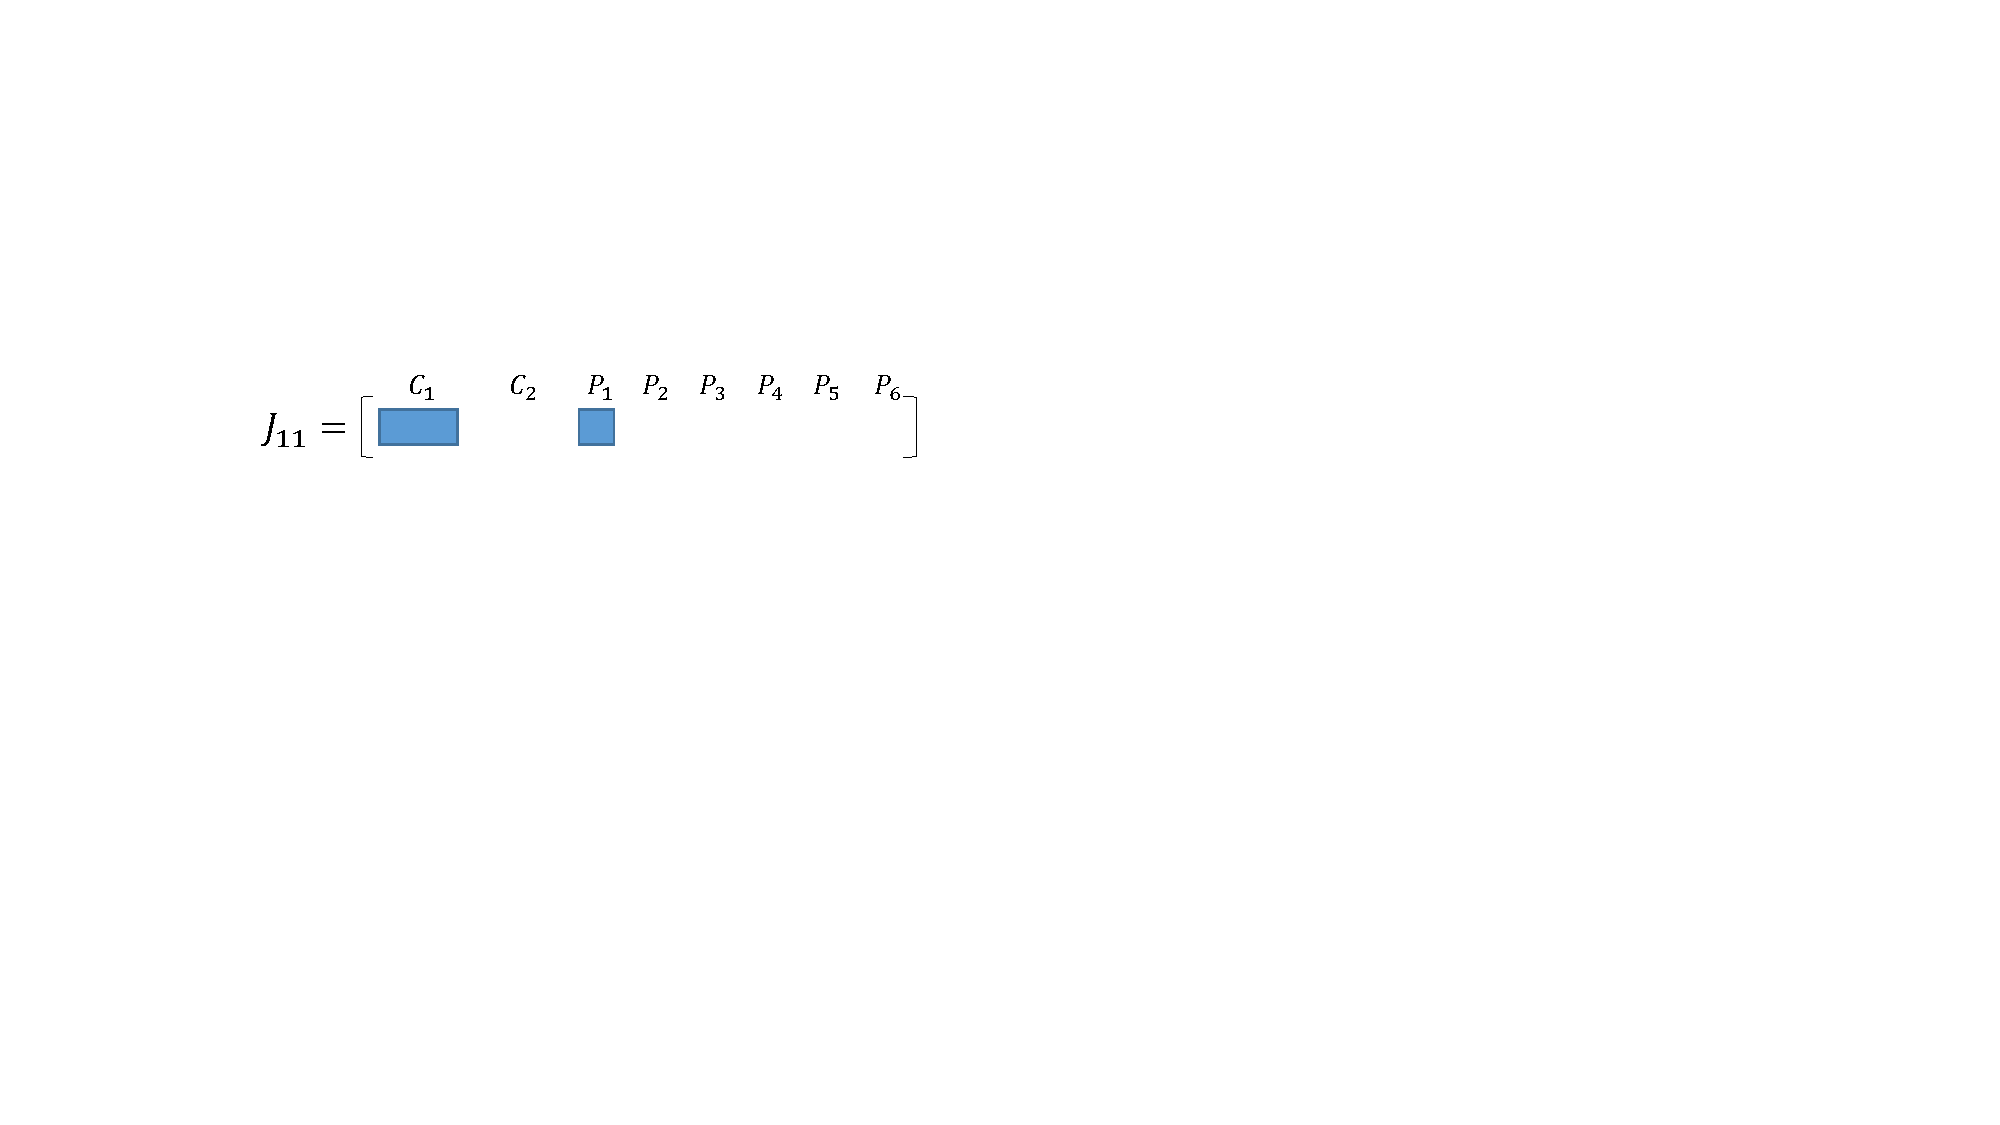
\includegraphics[width=0.8\textwidth]{backend1/Jacobianrow.pdf}
	\caption{The distribution of non-zero blocks of the $\mathbf{J}_{11}$ matrix. The upper mark indicates the variable corresponding to that column of the matrix. Since the pose dimension is larger than the landmark dimension, the matrix block corresponding to $C_1$ is wider than the matrix block corresponding to $P_1$.}
	\label{fig:jaobianrow}
\end{figure}
In order to obtain the Jacobian matrix corresponding to the objective function, we can list these $\mathbf{J}_{ij}$ as vectors in a certain order, then the overall Jacobian matrix and the corresponding $\mathbf{H}$ matrix The sparse situation is as shown in \autoref{fig:simplematrix}~.

\begin{figure}[!t]
	\centering
	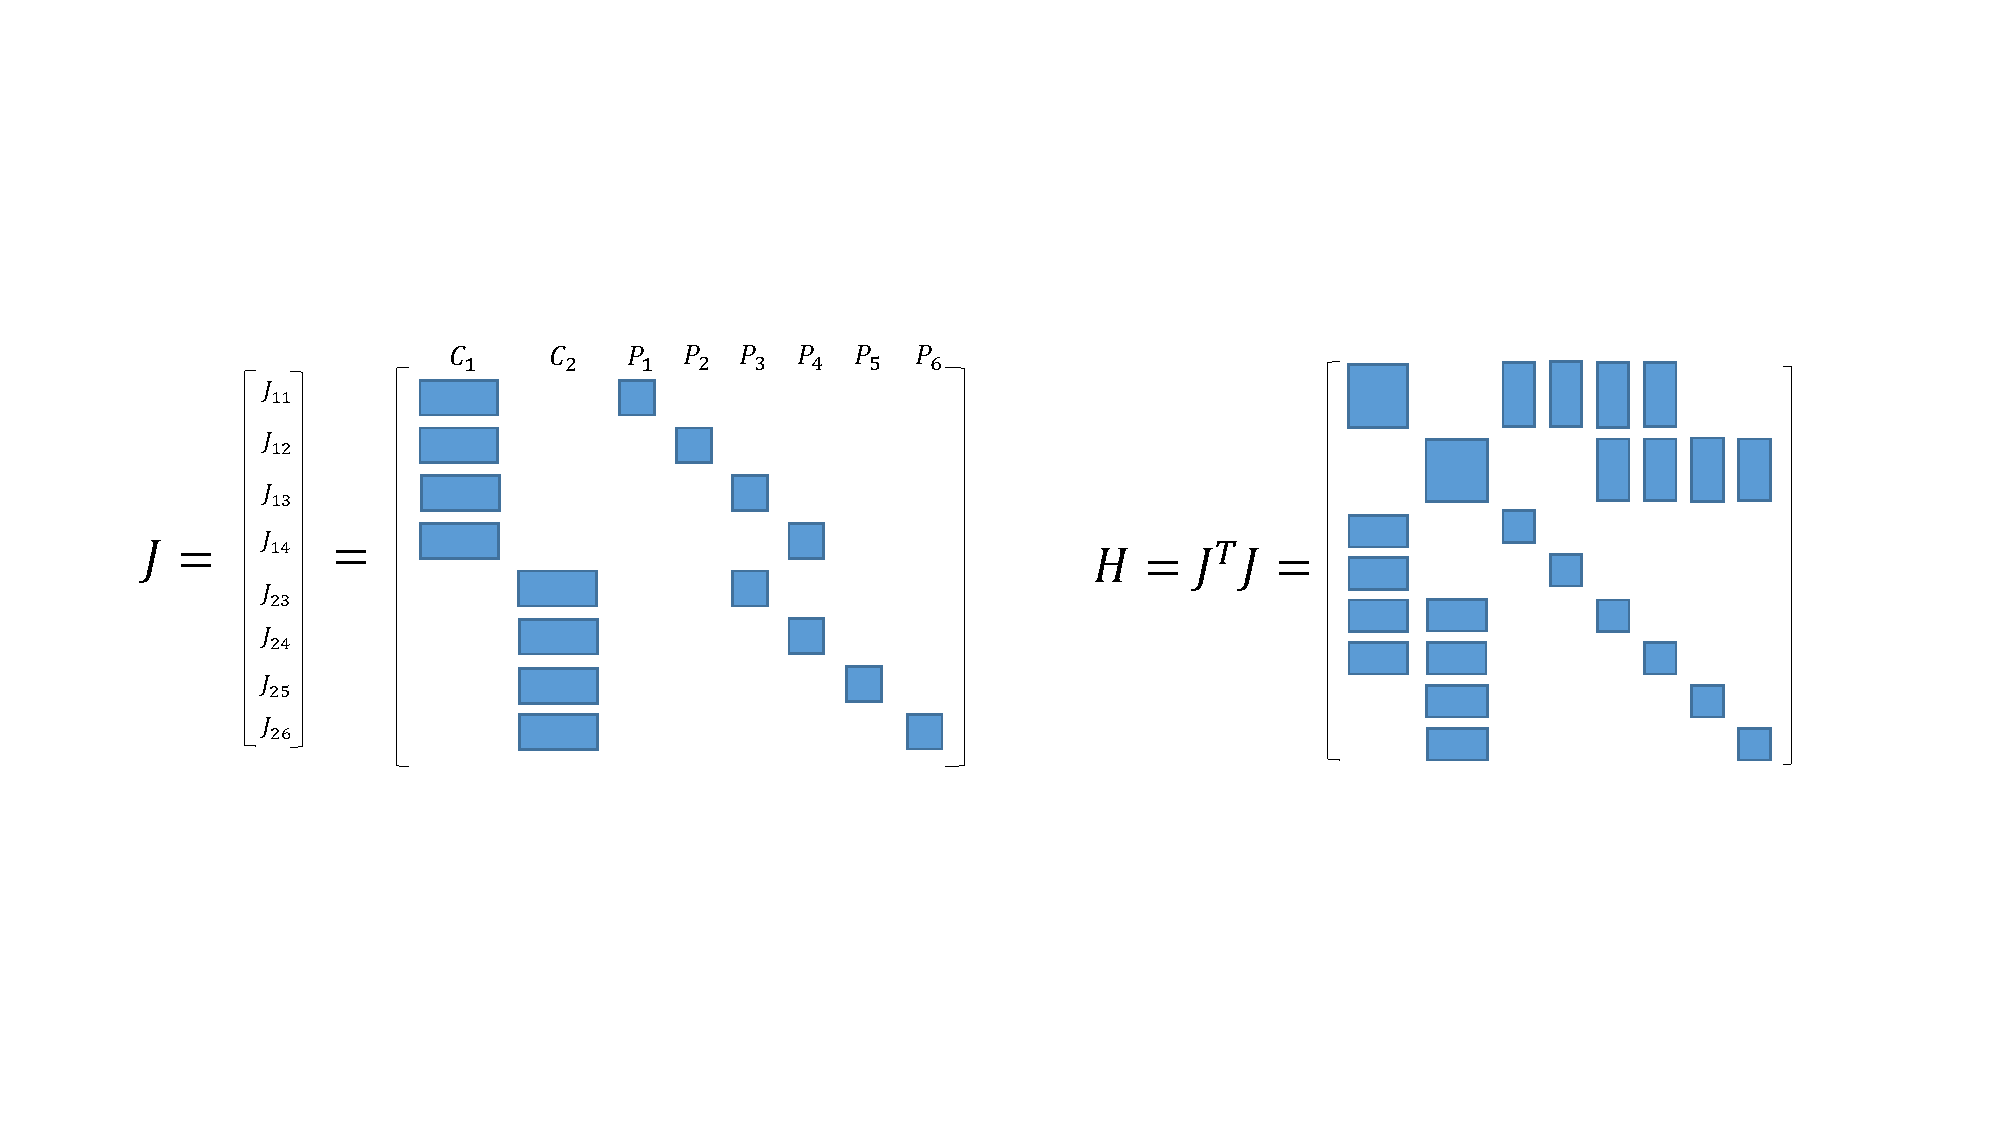
\includegraphics[width=1\textwidth]{backend1/simplematrix.pdf}
	\caption{The sparsity of the Jacobian matrix (left) and the sparsity of the $\mathbf{H}$ matrix (right). The colored squares indicate that the matrix has a non-zero value in the corresponding matrix block, and the rest of the uncolored parts indicate that the value of is always 0.}
	\label{fig:simplematrix}
\end{figure}

You may have noticed that the Hessian matrix in the \autoref{fig:simplegraph}~ has the same structure with the corresponding \textit{adjacency matrix} of the graph \footnote{The adjacency matrix is such a matrix that, its $i,j$ element describes whether there is a connected edge at nodes $i$ and $j$. If this edge exists, we set this element to 1, otherwise set to 0.} The above $\mathbf{H}$ matrix has a total of $8 \times 8$ matrix blocks. For the non-diagonal matrix block in the $\mathbf{H}$ matrix, if the matrix block is non-zero, then There will be an edge in the graph between the variables corresponding to their positions. We can clearly see this from \autoref{fig:matrixandgraph}~. Therefore, the non-zero matrix block in the non-diagonal part of the $\mathbf{H}$ matrix can be understood as a connection between its corresponding two variables, or it can be called a constraint. Therefore, we found that the graph optimization structure is obviously related to the sparsity of the incremental equation.

\begin{figure}[!htp]
	\centering
	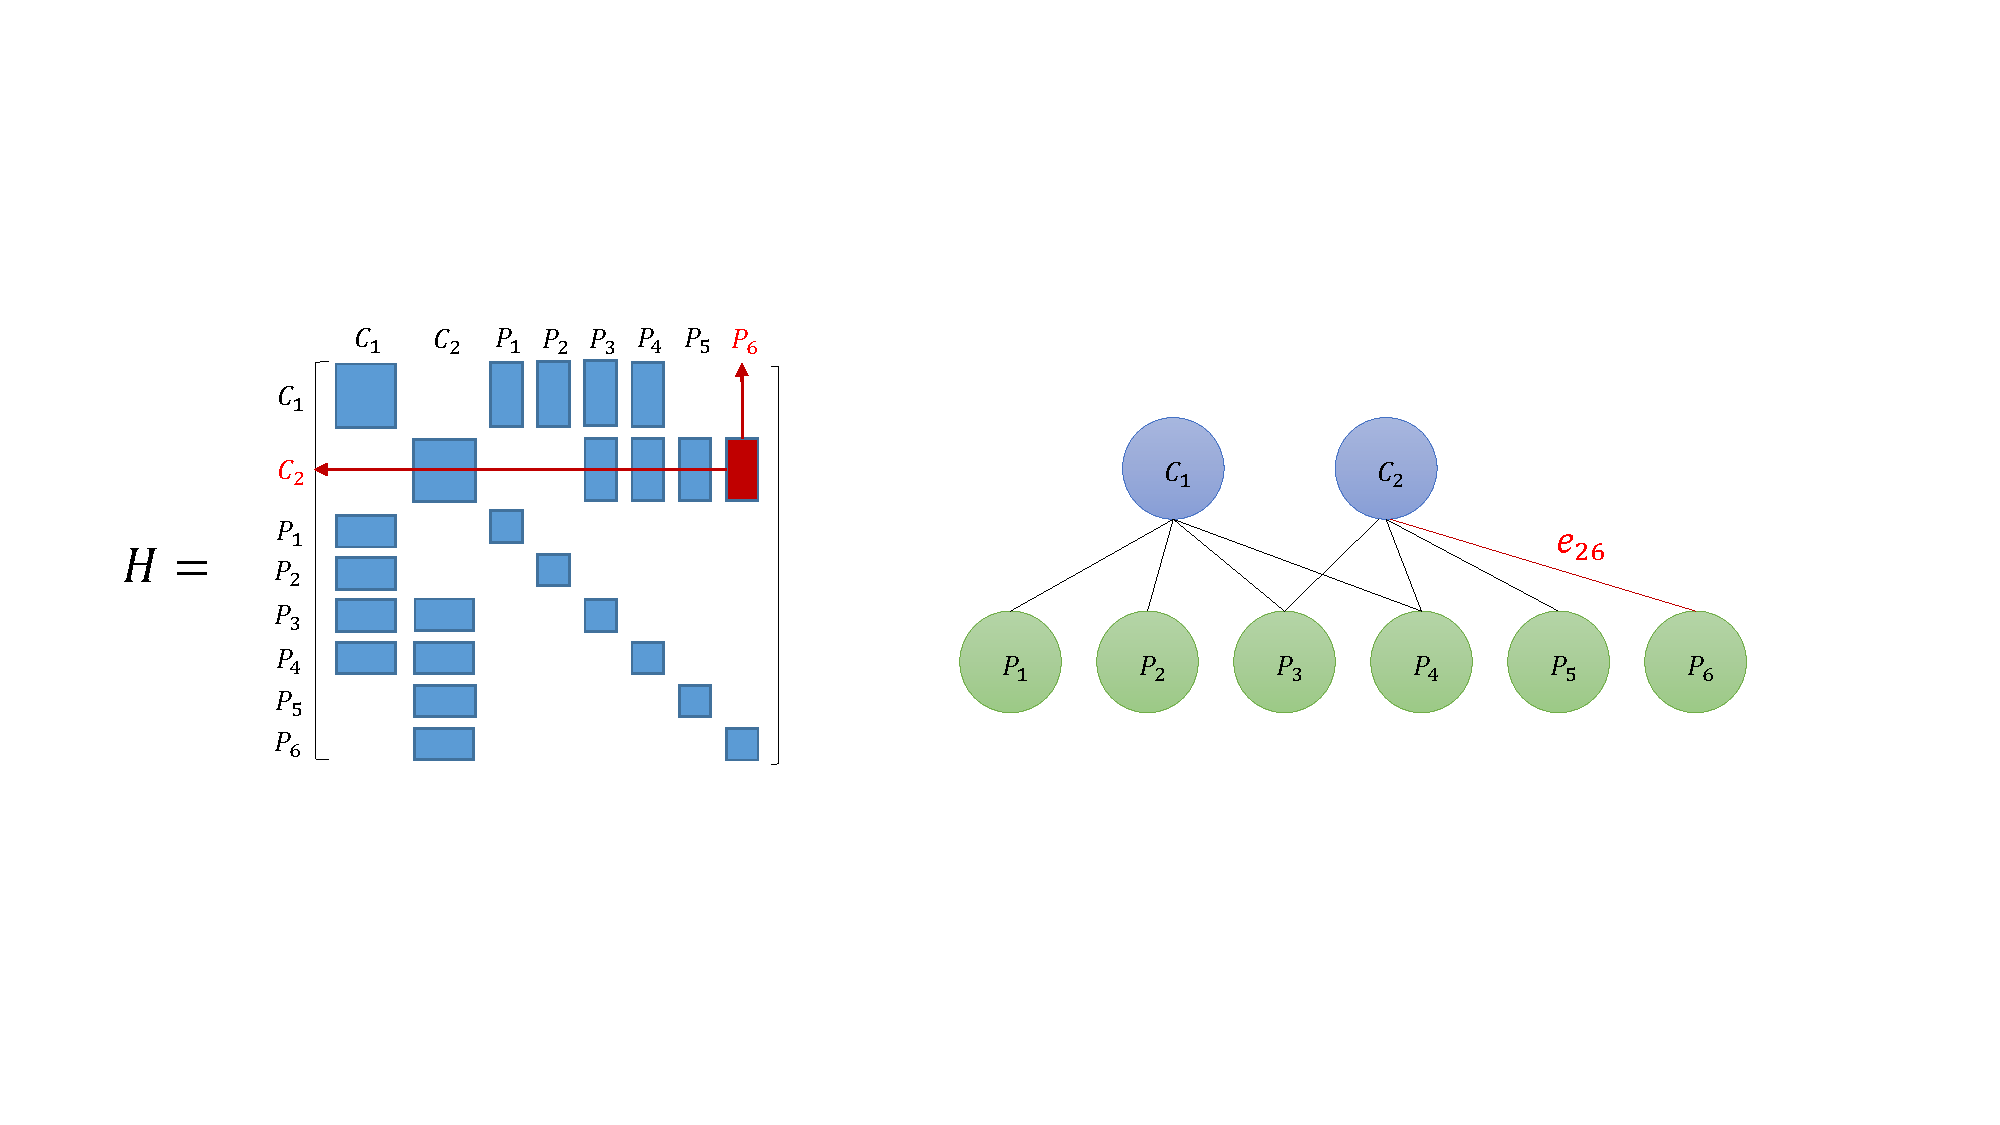
\includegraphics[width=1\textwidth]{backend1/matrixandgraph.pdf}
	\caption{The corresponding relationship between the non-zero matrix blocks in the $\mathbf{H}$ matrix and the edges in the graph. For example, the red matrix block on the right in the $\mathbf{H}$ matrix in the left picture indicates that there is an edge between the corresponding variables $C_2$ and $P_6$ in the right picture $\mathbf{e}_{26} $.}
	\label{fig:matrixandgraph}
\end{figure}

Now consider the more general situation, suppose we have $m$ camera poses and $n$ landmarks. Since there are usually far more landmarks than cameras, we have $n \gg m$. From the above reasoning, the actual $\mathbf{H}$ matrix will be something like in \autoref{fig:BigHmatrix}~. Its upper left corner block appears to be very small, while the lower right corner diagonal block takes up a lot of space. In addition, the non-diagonal part is distributed with scattered observation data. Because its shape is very similar to an arrow, it is also called an arrow-like matrix {\cite{Barfoot2016}}. At the same time, it is also very similar to a pickaxe in Minecraft, so I also call it a pickaxe matrix \footnote{This is just a joke, please do not write it like this in formal academic papers. }.

\begin{figure}[!ht]
	\centering
	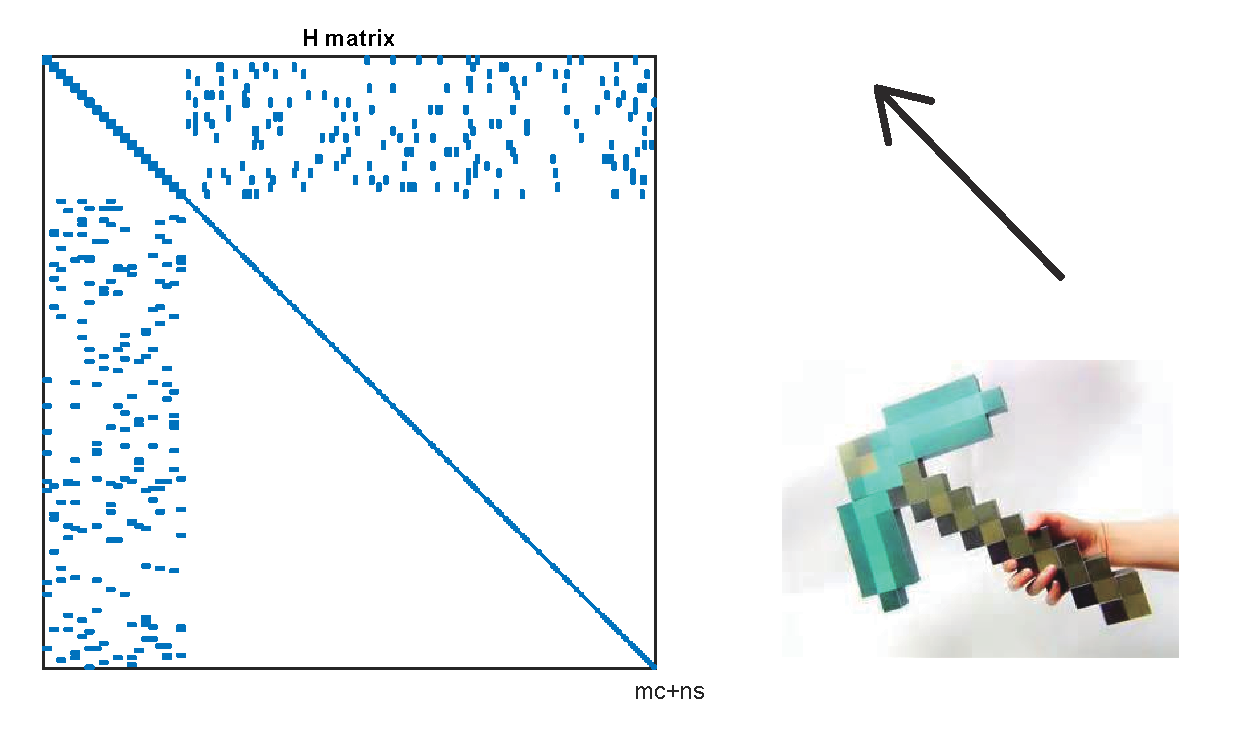
\includegraphics[width=0.7\textwidth]{backend1/BigHmatrix.pdf}
	\caption{$\mathbf{H}$ matrix in general cases.}
	\label{fig:BigHmatrix}
\end{figure}

\subsection{Schur Trick}
For $\mathbf{H}$ with this sparse structure, what is the difference in the solution of the linear equation $\mathbf{H} \Delta \mathbf{x}= \mathbf{g}$? In fact, there are several ways to use the sparsity of $\mathbf{H}$ to accelerate the calculations. This section introduces one of the most commonly used methods in visual SLAM: Schur elimination, also known as \textit{marginalization} in SLAM research.

Take a closer look at \autoref{fig:BigHmatrix}, we can easily find that this matrix can be divided into 4 blocks, which is consistent with \eqref{eq:H-blocks}. The upper left corner is a block-diagonal matrix, and the dimension of each block is the same as the dimension of the camera pose. The bottom-right corner is also a diagonal block matrix, and the dimension of each diagonal block is same as the dimension of the landmark. The structure of the off-diagonal block is related to the specific observation data. We first divide this matrix into regions as shown in \autoref{fig:MatrixSegmentation}. Readers can easily find that these 4 regions correspond to the 4 matrix blocks in the formula \eqref{eq:HessianMatrix}. For the convenience of subsequent analysis, we note these 4 blocks as $\mathbf{B}, \mathbf{E}, \mathbf{E}^T, \mathbf{C}$.

\begin{figure}[!ht]
	\centering
	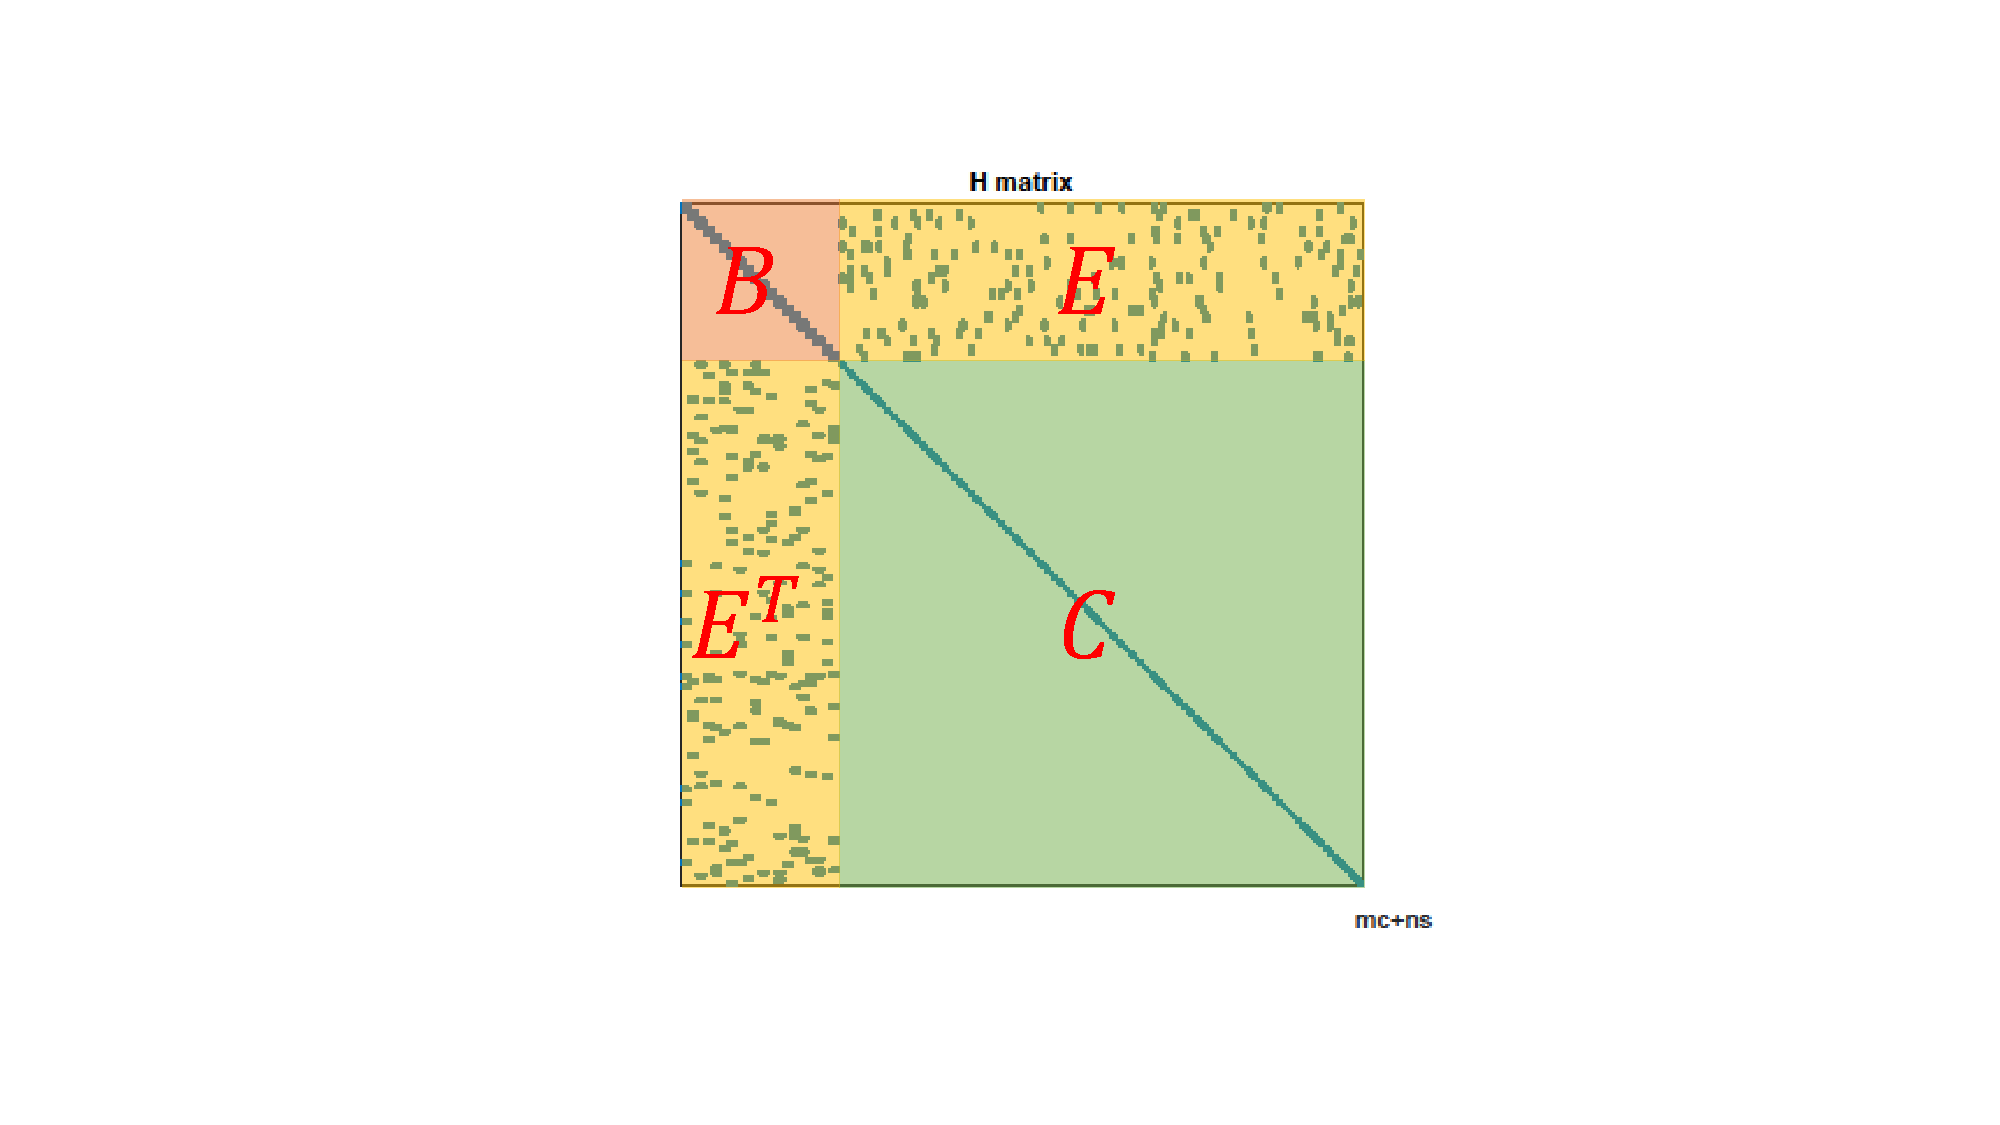
\includegraphics[width=0.5\textwidth]{backend1/MatrixSegmentation.pdf}
	\caption{Blocks in $\mathbf{H}$ matrix.}
	\label{fig:MatrixSegmentation}
\end{figure}

The linear equations $\mathbf{H\Delta x} = \mathbf{g}$ can be rewritten as: 
\begin{equation}
	\label{eq:linearequations}
	\left[ \begin{matrix}
		\mathbf{B}   &   \mathbf{E} \\
		\mathbf{E^T} &   \mathbf{C}
	\end{matrix}\right] 
	\left[ \begin{array}{l}
		\Delta \mathbf{x}_c \\
		\Delta \mathbf{x}_p 
	\end{array} \right] = 
	\left[ \begin{array}{l}
		\mathbf{v} \\
		\mathbf{w} 
	\end{array} \right],
\end{equation}
where $\mathbf{B}$ is a block-diagonal matrix. The dimension of each diagonal block is the same as the dimension of the camera poses. The number of diagonal blocks is the number of camera variables. Since the number of landmarks will be much larger than the number of camera variables, $\mathbf{C}$ is often much larger than $\mathbf{B}$. Since we use 3D landmarks, the $\mathbf{C}$ matrix is a diagonal block matrix wich each block beging a $3 \times 3$ matrix. The difficulty of inverting a diagonal block matrix is much less than that of a general matrix, because we only need to invert those diagonal blocks separately. Taking this feature into account, we perform Gaussian elimination on the linear equations. The goal is to eliminate the non-diagonal part $\mathbf{E}$ in the upper right corner, so we multiply a coefficient matrix on the left side: 
\begin{equation}\label{eq:guasselimination}
	\left[ \begin{matrix}
		\mathbf{I}   &    -\mathbf{EC^{-1}} \\
		\mathbf{0}	 &	  \mathbf{I}
	\end{matrix}\right]
	\left[ \begin{matrix}
		\mathbf{B}   &   \mathbf{E} \\
		\mathbf{E^T} &   \mathbf{C}
	\end{matrix}\right] 
	\left[ \begin{array}{l}
		\Delta \mathbf{x}_c \\
		\Delta \mathbf{x}_p 
	\end{array} \right] = 
	\left[ \begin{matrix}
		\mathbf{I}   &    -\mathbf{EC^{-1}}  \\
		\mathbf{0}	 &	  \mathbf{I}
	\end{matrix}
	\right]
	\left[ \begin{array}{l}
		\mathbf{v} \\
		\mathbf{w} 
	\end{array} \right]  .
\end{equation}

Rearrange it: 
\begin{equation}
	\left[ \begin{matrix}
		\mathbf{B} - \mathbf{E}\mathbf{C}^{-1}\mathbf{E}^T	& 	\mathbf{0} \\
		\mathbf{E}^T							& 	\mathbf{C}
	\end{matrix} \right]
	\left[ \begin{array}{l}
		\Delta \mathbf{x}_c \\
		\Delta \mathbf{x}_p 
	\end{array} \right] = 
	\left[\begin{array}{l}
		\mathbf{v} - \mathbf{E}\mathbf{C}^{-1}\mathbf{w}  \\
		\mathbf{w}
	\end{array}\right].
\end{equation}

After the elimination, the first line of the equations becomes a term that has nothing to do with $\Delta \mathbf{x}_p$. Take it out separately and get the incremental equation about the pose part:
\begin{equation}\label{eq:marginalization}
	\left[ 
	\mathbf{B} - \mathbf{E}\mathbf{C}^{-1}\mathbf{E}^T
	\right]
	\Delta \mathbf{x}_c  = 
	\mathbf{v} - \mathbf{E}\mathbf{C}^{-1}\mathbf{w} .
\end{equation}

The dimension of this linear equation is the same as the $\mathbf{B}$ matrix, and is much smaller than the overall equations. The Schur trick is to solve this equation first, then substitute the solved $\Delta \mathbf{x}_c$ into the original equation, and then solve $\Delta \mathbf{x}_p$. This process is called \textit{marginalization} {\cite{Sibley2010}}, or \textit{Schur elimination} (Schur trick). Compared with the method of directly solving linear equations, it have several obvious advantages:

\begin{enumerate}
	\item Since $\mathbf{C}$ is a block diagonal matrix, $\mathbf{C}^{-1}$ is easy to solve.
	\item After solving $\Delta \mathbf{x}_c$, the incremental equation of the landmark part is given by $\Delta \mathbf{x}_p = \mathbf{C}^{-1} (\mathbf{w}-\mathbf {E}^T \Delta \mathbf{x}_c)$. This still uses the easy-to-solve feature of $\mathbf{C}^{-1}$.
\end{enumerate}

Therefore, the main amount of calculation for marginalization is to solve the equation \eqref{eq:marginalization}. There is not much we can say about this equation. It is just an ordinary linear equation, no special structure can be used. Let us denote the coefficient of this equation as $\mathbf{S}$. How about its sparsity? \autoref{fig:marginalization} shows an instance of $\mathbf{S}$ after Schur elimination. It can be seen that its sparsity is somehow irregular.

\begin{figure}[!ht]
	\centering
	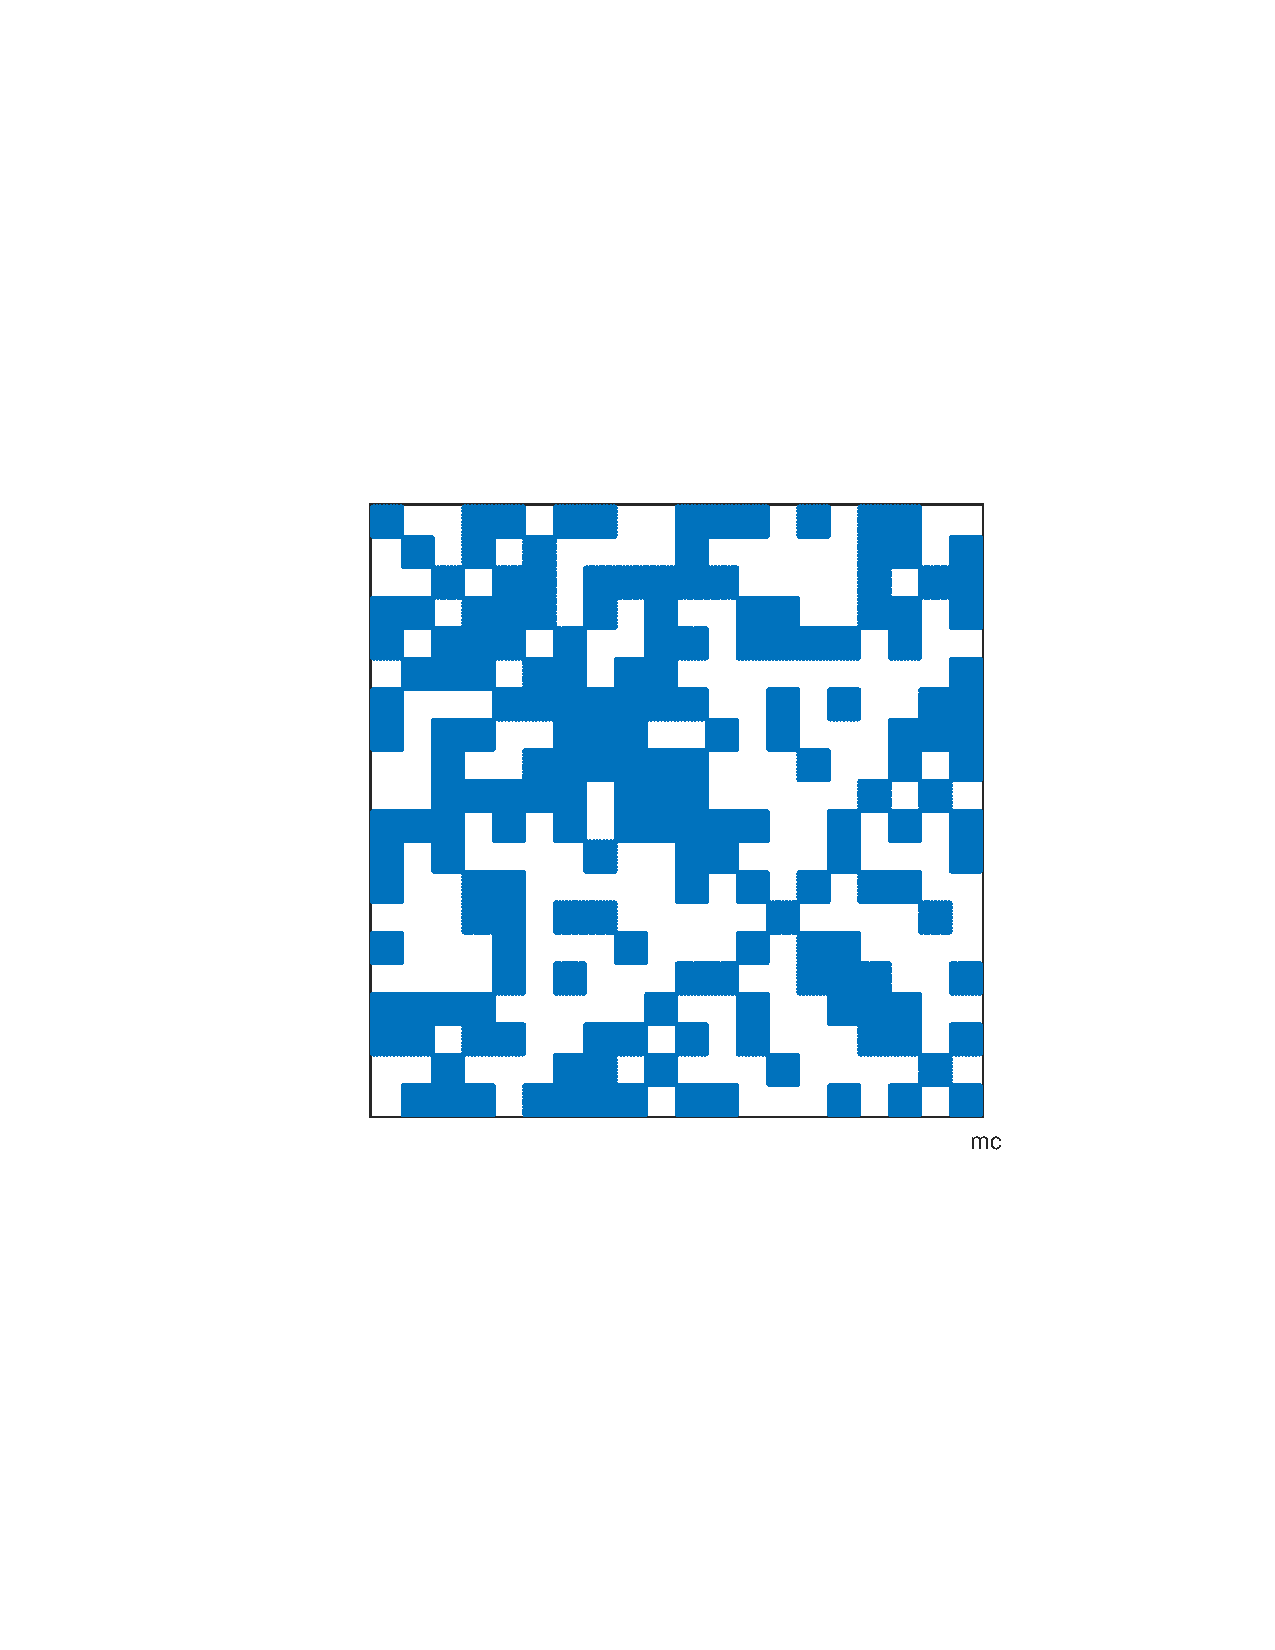
\includegraphics[width=0.5\textwidth]{backend1/marginalization.pdf}
	\caption{The sparse structure of the $\mathbf{S}$ matrix after Schur elimination. It looks like a QR code. Don't scan it.}
	\label{fig:marginalization}
\end{figure}

As mentioned earlier, the non-zero elements at the non-diagonal blocks of the $\mathbf{H}$ matrix correspond to the association between the camera and the landmark. Then, do the sparsity of $\mathbf{S}$ have physical meaning after Schur elimination? The answer is yes. Here we say without proof that the non-zero matrix block on the off-diagonal line of the $\mathbf{S}$ matrix indicates that there is a co-observation between the two camera variables. It is called \textit{co-visibility}. Conversely, if the block is zero, it means that the two cameras do not share any observation. For example, in the sparse matrix shown in \autoref{fig:marginalizationanalysis}~, the first $4 \times 4$ matrix blocks in the upper left corner can indicate that there are common observations between the corresponding camera variables $C_1, C_2, C_3$, and $C_4$.

\begin{figure}[!htp]
	\centering
	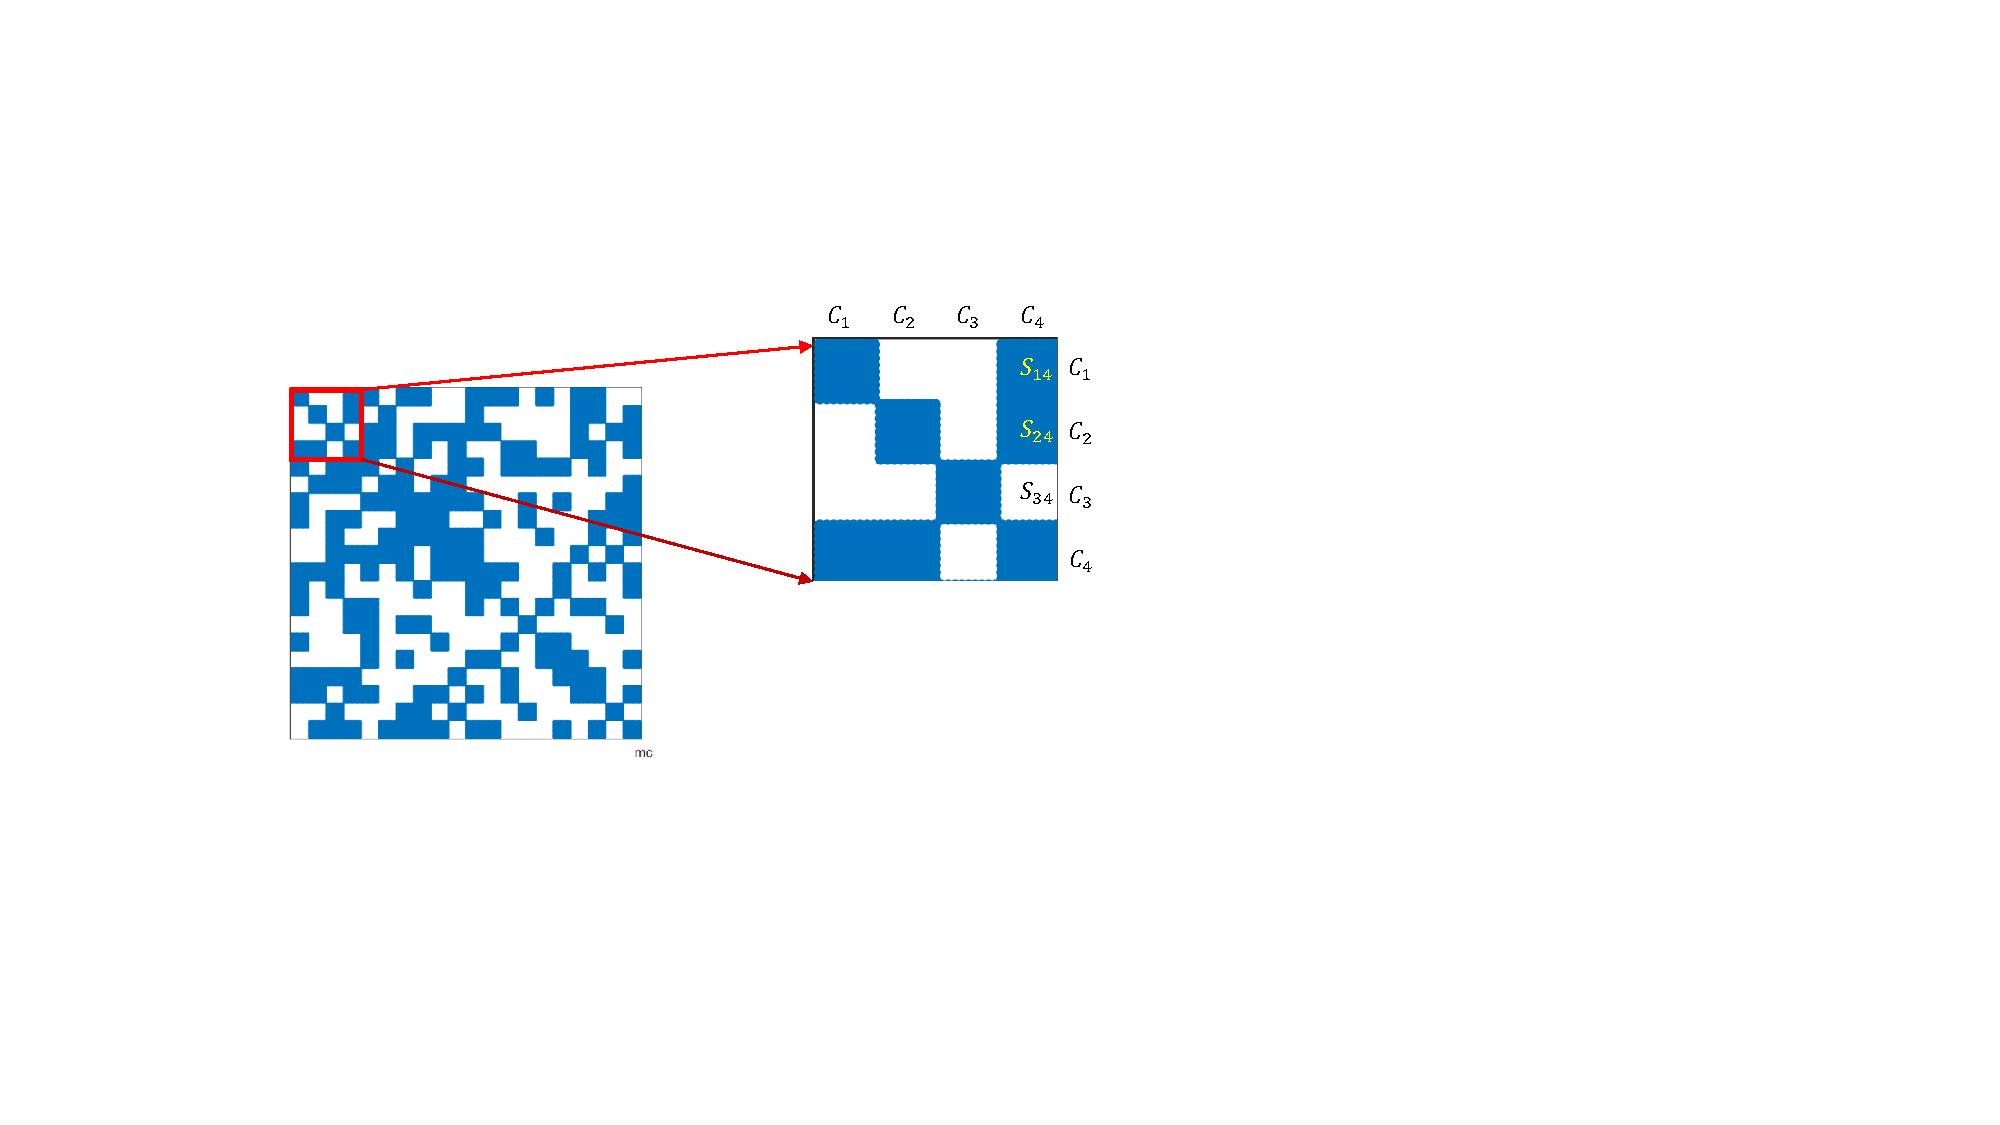
\includegraphics[width=0.8\textwidth]{backend1/marginalizationanalysis.pdf}
	\caption{Take the first $4 \times 4$ matrix blocks in the $\mathbf{S}$ matrix as an example, the matrix blocks in this area $\mathbf{S}_{14}, \mathbf{S}_{24}$ are not zero, meaning that there is at least one common observation between the camera $C_4$ and the cameras $C_1$ and $C_2$. Meanwhile, $S_{34}$ is zero means that there is no common observation between $C_3$ and $C_4$.}
	\label{fig:marginalizationanalysis}
\end{figure}

Therefore, the sparsity structure of the $\mathbf{S}$ matrix depends on the actual observation results, which we cannot predict in advance. In practice, for example, in the local mapping module of ORB-SLAM {\cite{Mur-Artal2015}}, we may deliberately select those frames with co-observations as keyframes, in this case the resulting $\mathbf{S}$ is a dense matrix. However, since this module is not executed in real time (normally runs in a separate thread in the backend), this approach is also acceptable. But in other methods, such as DSO {\cite{Engel2016}}, OKVIS {\cite{Leutenegger2015}}, etc., they use the sliding window method. Such methods will use the previous $\mathbf{S}$ matrix as a prior constraint in the following BA steps, so they must use some techniques to maintain the sparsity of the $\mathbf{S}$ matrix by discarding some observations. Readers who want to go deeper into this area can refer to their papers. I won't talk about these detailed things here.

From a probabilistic persepctive, we call this step as \textit{marginalization} because we actually converted the problem of seeking $(\Delta \mathbf{x}_c, \Delta \mathbf{x}_p)$ into fixing  $\Delta \mathbf{x}_p$ first, and finding $\Delta \mathbf{x}_c$, and then finding $\Delta \mathbf{x}_p$. This step is equivalent to the conditional probability expansion:
\begin{equation}
	\underbrace{P( \mathbf{x}_c, \mathbf{x}_p )}_{\text{joint}} = \underbrace{P(\mathbf{x}_c | \mathbf{x}_p )}_{\text{conditional}} \underbrace{P( \mathbf{x}_p )}_{\text{marginal}} ,
\end{equation}

The result is to convert a joint distribution to a multiplication of a conditional distribution and marginal distribution. In the previous sparse BA process, we actually marginalized all the landmarks. But we can also choose which part to marginalization according to the actual situation. Please also note that Schur elimination is only one way to achieve marginalization, and Cholesky decomposition can also be used for marginalization.

Readers may continue to ask, after the Schur elimination, we still need to solve the linear equations \eqref{eq:marginalization}. Are there any techniques for solving it? Unfortunately, this part belongs to the traditional numerical matrix solution, which is usually calculated by matrix decomposition. No matter which solution method is adopted, we recommend using the sparsity of $\mathbf{H}$ to perform Schur elimination first. This is not only because this can increase the speed, but also because the condition number of the $\mathbf{S}$ matrix after elimination is often smaller than the previous $\mathbf{H}$ matrix. Note that Schur elimination does not only mean to eliminate the landmarks. Eliminating camera variables is also a common method used in SLAM.

\subsection{Robust Kernels}
In the previous BA problem, we minimize the $\mathcal{L}_2$ norm of the error term in the objective function. Although this approach is intuitive, there is a serious problem: what happens if the data given by a certain error term is wrong for reasons such as mismatch? We added an edge that shouldn't have been added to the graph. However, the optimization algorithm does not know that this is wrong data. It will treat all data as noisy observations. From the point of view of the algorithm, this is equivalent to that we find an observation almost impossible to happen. At this time, there will be an edge with large error in graph optimization, and its gradient is also large, which means that adjusting the variables related to it will make the objective function drop more. Therefore, the algorithm will try to adjust the estimated value of the nodes connected by this edge first to make them comply with the unreasonable requirements of this edge. Since the error of this edge is really large, it tends to eliminate out the influence of other correct edges, making the optimization algorithm focus on adjusting a wrong value. This is obviously not what we want to see.

The reason for this problem is that when the error is large, the $\mathcal{L}_2$ norm grows too fast. So people propose something called kernel functions. The kernel function guarantees that the error of each edge will not be too big to cover up the other edges. The specific method is to replace the original  $\mathcal{L}_2$ norm metric of error with a function that does not grow that fast, while ensuring its own smoothness (otherwise we cannot compute derivatives). Because they make the overall optimization result more robust, they are also called robust kernel.

There are many kinds of robust kernel functions, such as the most commonly used Huber kernel:
\begin{equation}
	H\left( e \right) = 
	\left\{ 
	\begin{array}{ll}
		\frac{1}{2}{e^2} &\quad \text{when} |e| \leqslant \delta, \\
		\delta \left( {\left| e \right| - \frac{1}{2}\delta } \right) &\quad \text{otherwise}
	\end{array} \right.
\end{equation}

We see that when the error of $e$ is greater than a certain threshold $\delta$, the function growth changes from a quadratic form to a linear form, which is equivalent to limiting the maximum value of the gradient. At the same time, the Huber kernel function is smooth and can be easily derived. \autoref{fig:huber}~ shows the comparison between Huber's kernel function and the quadratic function. It can be seen that the growth of Huber's kernel function is significantly lower than that of the quadratic function when the error is large.

\begin{figure}[!htp]
	\centering
	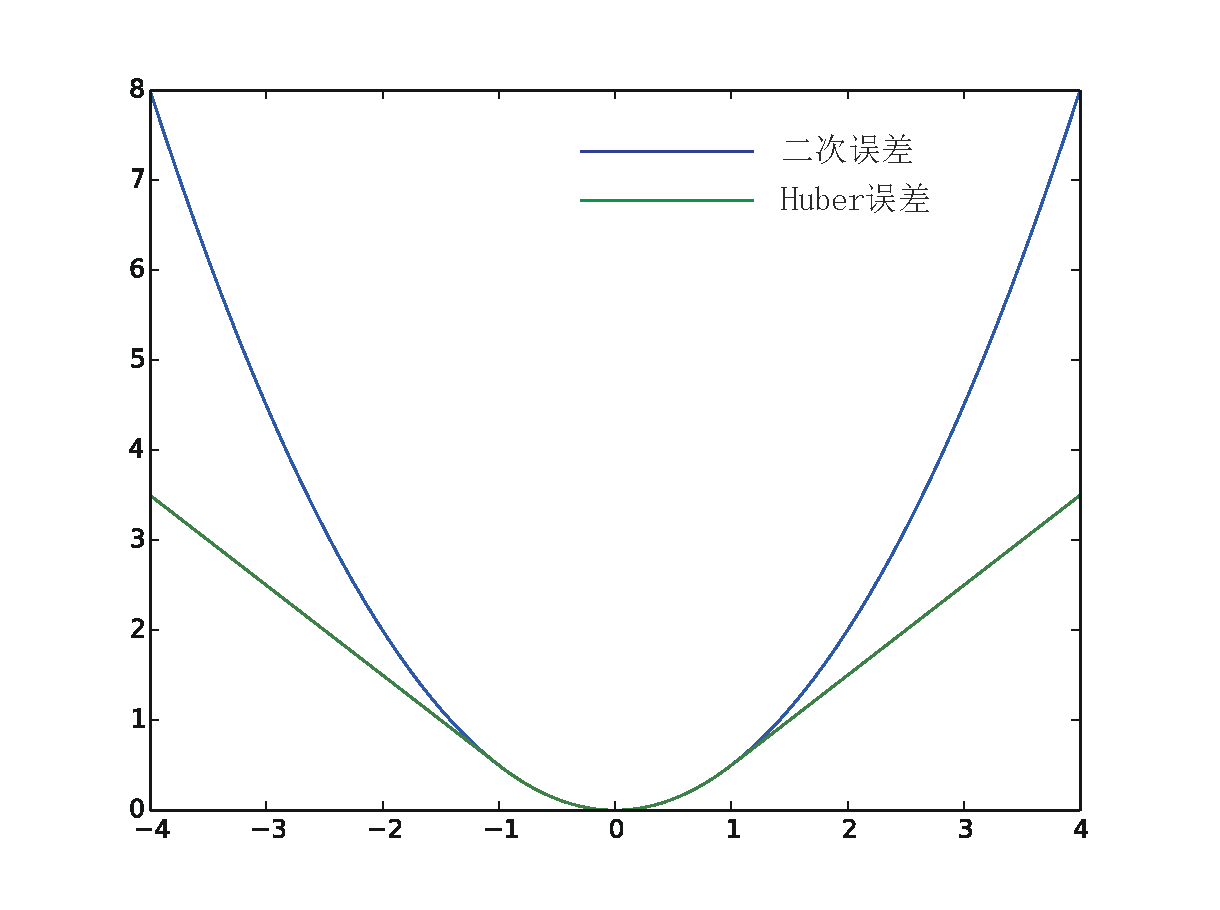
\includegraphics[width=0.5\textwidth]{backend1/huberloss}
	\caption{The Huber kernel.}
	\label{fig:huber}
\end{figure}

In addition to Huber kernels, there are also Cauchy kernels, Tukey kernels, and so on. Please check which kernel functions are supported in \textit{g2o} and \textit{Ceres}.

\subsection{Summary}
In this section, we focus on the sparsity problem in BA. However, in practice, most libraries have implemented the detailed operations for us, and what we need to do is mainly to construct the Bundle Adjustment problem, set the marginalized part, and then call the dense or sparse matrix solver to optimize the variables. If readers want to have a deeper understanding of BA, please refer to the~\cite{Triggs2000} or other related papers.

In the following two sections, we will use the Ceres and \textit{g2o} libraries to do Bundle Adjustment. In order to show the difference between them, we will use a public data set BAL~\cite{bundleadjustmentinlarge}, and use the common read and write code.

\section{Practice: BA with Ceres}
\subsection{BAL Dataset}
We use the BAL data set to demonstrate the BA experiments. The BAL data set provides several scenes. The camera and landmark information in each scene are given by a text file. We use the file problem-16-22106-pre.txt as an example. This file stores the BA problem information in a line-by-line manner. For the detailed format, see \url{https://grail.cs.washington.edu/projects/bal}. We use the BALProblem class defined in common.h to read in the content of the file, and then use Ceres and \textit{g2o} to solve them.

It should be noted that the BAL data set has some special features:
\begin{enumerate}
	\item  The camera intrinsic model of BAL is given by the focal length $f$ and the distortion parameters $k_1,k_2$, where $f$ is same as the $f_x$ and $f_y$ mentioned before. Since the pixels of the photo are basically square, in many practical situations, $f_x$ is very close to $f_y$, so it is possible to use the same value. In addition, there is no $c_x, c_y$ in this model, because these two values have been removed from the stored data.
	\item BAL data assumes that the projection plane is behind the optical center of the camera when projecting, so if we calculate according to the model we used before, we need to multiply $-1$ after projection. However, most data sets still use the projection plane in front of the optical center. We should read the format description carefully before using the data set.
\end{enumerate}

After reading the data with the BALProblem class, we can call the Normalize function to normalize the original data, or add noise to the data through the Perturb function. Normalization means setting zero to the centers of all landmarks, and then scaling them to an appropriate scale. This will make the value in the optimization process more stable and prevent BA to get very large values in extreme cases.

Please read the other interfaces of the BALProblem class by yourself. Since these codes are only responsible for IO functions, in order to save space, we will not print them in the text. After solving the BA, we can also use this type of function to write the result into a ply file (a point cloud file format), and then use the meshlab software to view it. Meshlab can be installed via apt-get, and the installation method is not described here.

\subsection{Solving BA in Ceres}
In the bundle\_adjustment\_ceres.cpp file, we implemented the process of solving BA in Ceres. The key to using Ceres is to define the projection error model. This part of the code is given in SnavelyReprojectionError.h:

\begin{lstlisting}[language=c++, caption=slambook2/ch9/SnavelyReprojectionError.cpp (part)]
class SnavelyReprojectionError {
public:
	SnavelyReprojectionError(double observation_x, double observation_y) : observed_x(observation_x), observed_y(observation_y) {}
	
	template<typename T>
	bool operator()(const T *const camera,
		const T *const point,
		T *residuals) const {
		// camera[0,1,2] are the angle-axis rotation
		T predictions[2];
		CamProjectionWithDistortion(camera, point, predictions);
		residuals[0] = predictions[0] - T(observed_x);
		residuals[1] = predictions[1] - T(observed_y);
		
		return true;
	}
	
	// camera : 9 dims array
	// [0-2] : angle-axis rotation
	// [3-5] : translation
	// [6-8] : camera parameter, [6] focal length, [7-8] second and forth order radial distortion
	// point : 3D location.
	// predictions : 2D predictions with center of the image plane.
	template<typename T>
	static inline bool CamProjectionWithDistortion(const T *camera, const T *point, T *predictions) {
		// Rodrigues' formula
		T p[3];
		AngleAxisRotatePoint(camera, point, p);
		// camera[3,4,5] are the translation
		p[0] += camera[3];
		p[1] += camera[4];
		p[2] += camera[5];
		
		// Compute the center fo distortion
		T xp = -p[0] / p[2];
		T yp = -p[1] / p[2];
		
		// Apply second and fourth order radial distortion
		const T &l1 = camera[7];
		const T &l2 = camera[8];
		
		T r2 = xp * xp + yp * yp;
		T distortion = T(1.0) + r2 * (l1 + l2 * r2);
		
		const T &focal = camera[6];
		predictions[0] = focal * distortion * xp;
		predictions[1] = focal * distortion * yp;
		
		return true;
	}
	
	static ceres::CostFunction *Create(const double observed_x, const double observed_y) {
		return (new ceres::AutoDiffCostFunction<SnavelyReprojectionError, 2, 9, 3>(
			new SnavelyReprojectionError(observed_x, observed_y)));
	}
	
private:
	double observed_x;
	double observed_y;
};
\end{lstlisting}
This overloaded bracket operator in this class implements the error calculation, whose main body is in the  CamProjectionWithDistortion function. Note that in Ceres, we must store optimized variables in the form of a double array. Now each camera has a total of 6-dimensional pose, 1-dimensional focal length, and 2-dimensional distortion parameters, which are described by a total of 9-dimensional parameters. We must also store them in this order in actual storage. The stati cCreate function of this class acts as an external interface that directly returns a Ceres cost function that can be automatically derived. We only need to call the Create function and put the cost function into ceres::Problem.

Next we realize the part of building and solving BA:
\begin{lstlisting}[language=c++, caption=slambook2/ch9/SnavelyReprojectionError.cpp (part)]
void SolveBA(BALProblem &bal_problem) {
	const int point_block_size = bal_problem.point_block_size();
	const int camera_block_size = bal_problem.camera_block_size();
	double *points = bal_problem.mutable_points();
	double *cameras = bal_problem.mutable_cameras();
	
	// Observations is 2 * num_observations long array observations
	// [u_1, u_2, ... u_n], where each u_i is two dimensional, the x
	// and y position of the observation.
	const double *observations = bal_problem.observations();
	ceres::Problem problem;
	
	for (int i = 0; i < bal_problem.num_observations(); ++i) {
		ceres::CostFunction *cost_function;
		
		// Each Residual block takes a point and a camera as input
		// and outputs a 2 dimensional Residual
		cost_function = 
		SnavelyReprojectionError::Create(observations[2 * i + 0], observations[2 * i + 1]);
		
		// If enabled use Huber's loss function.
		ceres::LossFunction *loss_function = new ceres::HuberLoss(1.0);
		
		// Each observation corresponds to a pair of a camera and a point
		// which are identified by camera_index()[i] and point_index()[i]
		// respectively.
		double *camera = cameras + camera_block_size * bal_problem.camera_index()[i];
		double *point = points + point_block_size * bal_problem.point_index()[i];
		
		problem.AddResidualBlock(cost_function, loss_function, camera, point);
	}
	
	std::cout << "Solving ceres BA ... " << endl;
	ceres::Solver::Options options;
	options.linear_solver_type = ceres::LinearSolverType::SPARSE_SCHUR;
	options.minimizer_progress_to_stdout = true;
	ceres::Solver::Summary summary;
	ceres::Solve(options, &problem, &summary);
	std::cout << summary.FullReport() << "\n";
}
\end{lstlisting} 

It can be seen that the problem building part is quite simple. If you want to add other cost functions, the entire process will not change much. Finally, in ceres::Solver::Options, we can set the solution method. Using SPARSE\_SCHUR will make the actual solution process of Ceres same as we described earlier, that is, first perform Schur marginalization on the landmarks to solve this problem in an accelerated manner. However, in Ceres we cannot control which part of the variables are marginalized, which is automatically searched and calculated by the Ceres solver.

The output of Ceres BA is like:
\begin{lstlisting}[language=sh,caption=Terminal output]
./build/bundle_adjustment_ceres  problem-16-22106-pre.txt                
Header: 16 22106 83718bal problem file loaded...
bal problem have 16 cameras and 22106 points. 
Forming 83718 observations. 
Solving ceres BA ... 
iter      cost      cost_change  |gradient|   |step|    tr_ratio  tr_radius  ls_iter  iter_time  total_time
0  1.842900e+07    0.00e+00    2.04e+06   0.00e+00   0.00e+00  1.00e+04        0    6.10e-02    2.24e-01
1  1.449093e+06    1.70e+07    1.75e+06   2.16e+03   1.84e+00  3.00e+04        1    1.79e-01    4.03e-01
2  5.848543e+04    1.39e+06    1.30e+06   1.55e+03   1.87e+00  9.00e+04        1    1.56e-01    5.59e-01
3  1.581483e+04    4.27e+04    4.98e+05   4.98e+02   1.29e+00  2.70e+05        1    1.51e-01    7.10e-01
......
\end{lstlisting}

The overall error should continue to decrease as the number of iterations increases. Finally, we output the point clouds before and after optimization as initial.ply and final.ply, which can be opened directly with meshlab. The result graph is shown in \autoref{fig:g2o-BA}.

\begin{figure}[!htp]
	\centering
	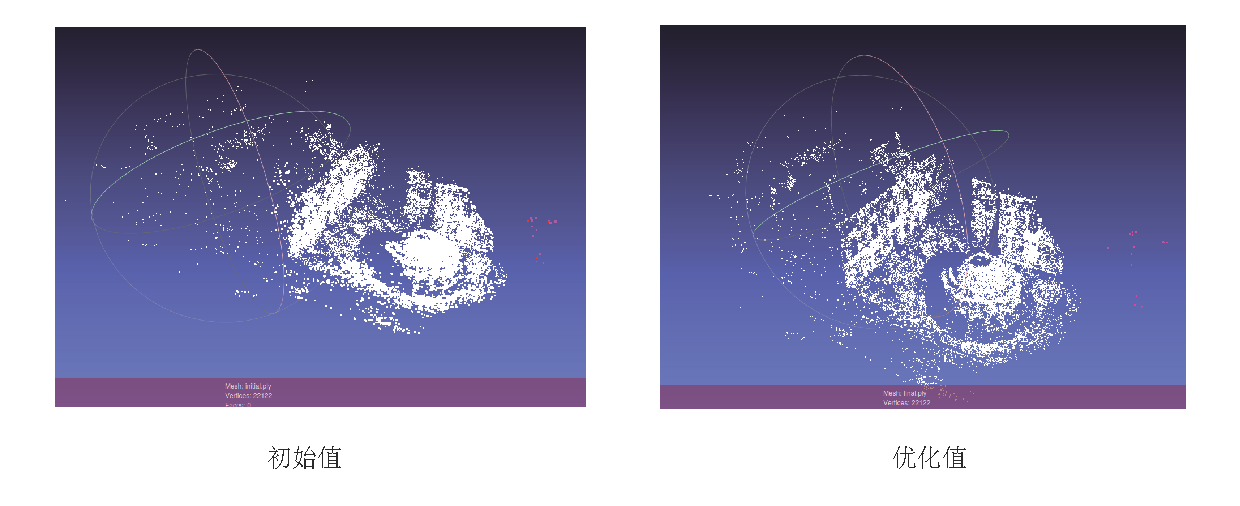
\includegraphics[width=1.0\textwidth]{backend1/g2o-BA}
	\caption{Visualized point cloud before and after optimization. Left side: the initial value before optimization; Right side: the optimized value.}
	\label{fig:g2o-BA}
\end{figure}

\section{Practice: BA with \textit{g2o}}
Let's consider how to use \textit{g2o} to solve this BA problem. As mentioned before, \textit{g2o} uses a graph model to describe the problem's structure, so we need to use nodes to represent cameras and landmarks and then use edges to represent observations between them. We still use custom defined vertices and edges instead of built-in edges. For cameras and landmarks, we can define the following structure and use the override keyword to indicate the virtual functions:

\begin{lstlisting}[language=c++,caption=slambook2/ch9/bundle_adjustment_g2o.cpp (part)]
struct PoseAndIntrinsics {
	PoseAndIntrinsics() {}
	
	/// set from given data address
	explicit PoseAndIntrinsics(double *data_addr) {
		rotation = SO3d::exp(Vector3d(data_addr[0], data_addr[1], data_addr[2]));
		translation = Vector3d(data_addr[3], data_addr[4], data_addr[5]);
		focal = data_addr[6];
		k1 = data_addr[7];
		k2 = data_addr[8];
	}
	
	/// set to double array
	void set_to(double *data_addr) {
		auto r = rotation.log();
		for (int i = 0; i < 3; ++i) data_addr[i] = r[i];
		for (int i = 0; i < 3; ++i) data_addr[i + 3] = translation[i];
		data_addr[6] = focal;
		data_addr[7] = k1;
		data_addr[8] = k2;
	}
	
	SO3d rotation;
	Vector3d translation = Vector3d::Zero();
	double focal = 0;
	double k1 = 0, k2 = 0;
};

/// pose and f, k1, k2
class VertexPoseAndIntrinsics : public g2o::BaseVertex<9, PoseAndIntrinsics> {
	public:
	EIGEN_MAKE_ALIGNED_OPERATOR_NEW;
	
	VertexPoseAndIntrinsics() {}
	
	virtual void setToOriginImpl() override {
		_estimate = PoseAndIntrinsics();
	}
	
	virtual void oplusImpl(const double *update) override {
		_estimate.rotation = SO3d::exp(Vector3d(update[0], update[1], update[2])) * _estimate.rotation;
		_estimate.translation += Vector3d(update[3], update[4], update[5]);
		_estimate.focal += update[6];
		_estimate.k1 += update[7];
		_estimate.k2 += update[8];
	}
	
	Vector2d project(const Vector3d &point) {
		Vector3d pc = _estimate.rotation * point + _estimate.translation;
		pc = -pc / pc[2];
		double r2 = pc.squaredNorm();
		double distortion = 1.0 + r2 * (_estimate.k1 + _estimate.k2 * r2);
		return Vector2d(_estimate.focal * distortion * pc[0],
		_estimate.focal * distortion * pc[1]);
	}
	
	virtual bool read(istream &in) {}
	virtual bool write(ostream &out) const {}
};

class VertexPoint : public g2o::BaseVertex<3, Vector3d> {
	public:
	EIGEN_MAKE_ALIGNED_OPERATOR_NEW;
	
	VertexPoint() {}
	
	virtual void setToOriginImpl() override {
		_estimate = Vector3d(0, 0, 0);
	}
	
	virtual void oplusImpl(const double *update) override {
		_estimate += Vector3d(update[0], update[1], update[2]);
	}
	
	virtual bool read(istream &in) {}
	
	virtual bool write(ostream &out) const {}
};

class EdgeProjection :
public g2o::BaseBinaryEdge<2, Vector2d, VertexPoseAndIntrinsics, VertexPoint> {
	public:
	EIGEN_MAKE_ALIGNED_OPERATOR_NEW;
	
	virtual void computeError() override {
		auto v0 = (VertexPoseAndIntrinsics *) _vertices[0];
		auto v1 = (VertexPoint *) _vertices[1];
		auto proj = v0->project(v1->estimate());
		_error = proj - _measurement;
	}
	
	// use numeric derivatives in g2o
	virtual bool read(istream &in) {}
	virtual bool write(ostream &out) const {}
};
\end{lstlisting}

We define the rotation, translation, focal length, and distortion parameters in the same camera vertex and then define the camera's observation edge and the landmark. Here we do not implement the Jacobian calculation function of the edge \footnote{You can implement it by yourself if interested. Here we just want to make a fair comparison since we do not provide Jacobians in Ceres version.}, so \textit{g2o} will automatically provide a numerical calculation of Jacobian. Finally, according to the data in BAL, we can set up the optimization problem of g2o:
\begin{lstlisting}[language=c++,caption=slambook2/ch9/bundle_adjustment_g2o.cpp (part)]
void SolveBA(BALProblem &bal_problem) {
	const int point_block_size = bal_problem.point_block_size();
	const int camera_block_size = bal_problem.camera_block_size();
	double *points = bal_problem.mutable_points();
	double *cameras = bal_problem.mutable_cameras();
	
	// pose dimension 9, landmark is 3
	typedef g2o::BlockSolver<g2o::BlockSolverTraits<9, 3>> BlockSolverType;
	typedef g2o::LinearSolverCSparse<BlockSolverType::PoseMatrixType> LinearSolverType;
	// use LM
	auto solver = new g2o::OptimizationAlgorithmLevenberg(
	g2o::make_unique<BlockSolverType>(g2o::make_unique<LinearSolverType>()));
	g2o::SparseOptimizer optimizer;
	optimizer.setAlgorithm(solver);
	optimizer.setVerbose(true);
	
	/// build g2o problem
	const double *observations = bal_problem.observations();
	// vertex
	vector<VertexPoseAndIntrinsics *> vertex_pose_intrinsics;
	vector<VertexPoint *> vertex_points;
	for (int i = 0; i < bal_problem.num_cameras(); ++i) {
		VertexPoseAndIntrinsics *v = new VertexPoseAndIntrinsics();
		double *camera = cameras + camera_block_size * i;
		v->setId(i);
		v->setEstimate(PoseAndIntrinsics(camera));
		optimizer.addVertex(v);
		vertex_pose_intrinsics.push_back(v);
	}
	for (int i = 0; i < bal_problem.num_points(); ++i) {
		VertexPoint *v = new VertexPoint();
		double *point = points + point_block_size * i;
		v->setId(i + bal_problem.num_cameras());
		v->setEstimate(Vector3d(point[0], point[1], point[2]));
		// in g2o we should manually set the marginalized part 
		v->setMarginalized(true);
		optimizer.addVertex(v);
		vertex_points.push_back(v);
	}
	
	// edge
	for (int i = 0; i < bal_problem.num_observations(); ++i) {
		EdgeProjection *edge = new EdgeProjection;
		edge->setVertex(0, vertex_pose_intrinsics[bal_problem.camera_index()[i]]);
		edge->setVertex(1, vertex_points[bal_problem.point_index()[i]]);
		edge->setMeasurement(Vector2d(observations[2 * i + 0], observations[2 * i + 1]));
		edge->setInformation(Matrix2d::Identity());
		edge->setRobustKernel(new g2o::RobustKernelHuber());
		optimizer.addEdge(edge);
	}
	
	optimizer.initializeOptimization();
	optimizer.optimize(40);
	
	// set to bal problem
	for (int i = 0; i < bal_problem.num_cameras(); ++i) {
		double *camera = cameras + camera_block_size * i;
		auto vertex = vertex_pose_intrinsics[i];
		auto estimate = vertex->estimate();
		estimate.set_to(camera);
	}
	for (int i = 0; i < bal_problem.num_points(); ++i) {
		double *point = points + point_block_size * i;
		auto vertex = vertex_points[i];
		for (int k = 0; k < 3; ++k) point[k] = vertex->estimate()[k];
	}
}
\end{lstlisting}

The above defines the nodes and edges used in this problem. Next, we need to generate some nodes and edges based on the actual data in the BALProblem class and hand them to \textit{g2o} for optimization. It is worth noting that to take full advantage of sparse BA, we must set the setMarginalized function in the landmarks here. The big difference between \textit{g2o} and Ceres is that when using sparse optimization, \textit{g2o} must manually set which vertices are marginalized; otherwise, it will report a runtime error (readers can try to comment out the v->setMarginalized(true) line). The rest is similar to the Ceres version, so that we won't introduce more. The g2o experiment will also output point clouds before and after optimization for comparison and review.

\section{Summary}
This lecture discusses the state estimation problem and the solution of graph optimization in depth. We see that SLAM can be regarded as a state estimation problem in the classic model. If we assume Markov property and only consider the current state, we get a filter model represented by EKF. If not, we can also choose to consider all motions and observations, which constitute a least-squares problem. In the case of only observation equations, this problem is called BA and can be solved by nonlinear optimization methods. We carefully discussed the sparsity problem in the solution process and pointed out the connection between the problem and graph optimization. Finally, we demonstrated how to use the \textit{g2o} and Ceres libraries to solve the same optimization problem so that readers have an intuitive understanding of BA.

\section*{Exercises}
\begin{enumerate}
	\item Derive \eqref{eq:kalman-K-another} using Sherman-Morrison-Woodbury identities~\cite{Sherman1950, Barfoot2016}.
	\item 
	Compare the final cost of \textit{g2o} and Ceres after optimization. Discuss why they are siminlar in Meshlab by have different numerical values.
	\item 
	Search for methods that can provide partial Schur elimination in Ceres, and show the difference. 
	\item Show that the $\mathbf{S}$ matrix is semi-definite. 
	\item Read~\cite{Kummerle2011} and discuss the difference between the kernel functions in \textit{g2o} and the loss function in Ceres.
	\item[\optional] In the practice part, we optimize the pose and intrinsics parametrized with $f, k_1, k_2$. Please use the full intrinsic and distortion model in lecture 5 and modify the programs to complete the optimization. 
\end{enumerate}

